\section{Analýza}
\noindent Našou úlohou v rámci tejto bakalárskej práce je navrhnúť a vytvoriť interaktívne animácie na tému \acrshort{IGBT} (Bipolárny tranzistor s izolovaným hradlom), ktoré budú  žiakom a študentom voľne dostupné. Interaktívnu animáciu môžeme zahrnúť do vzdelávania ako moderný spôsob edukácie. Pomocou interaktívnej animácie umožníme študentom aby sami získali vedomosti o tom, ako fungujú \acrshort{IGBT} tranzistory. Túto problematiku budeme riešiť rozdelením dôležitých informácií na jednotlivé kapitoly, tj podstránky, medzi ktorými si študent bude schopný preklikávať a učiť sa pomocou interakcie s našimi animáciami. Vďaka tomu veríme, že sa nám podarí zvýšiť záujem mladých študentov o elektrotechniku, lebo v posledných  rokoch ten záujem pomaly klesá.

\subsection{Analýza problému}
\noindent V kapitole analýza sa zaoberáme témami edukačnej interaktívnej animácie, grafickými možnosťami ako aj možnosťami na animovanie. Taktiež sa budeme venovať úvodným poznatkom o \acrshort{IGBT} tranzistoroch a objasníme,  prečo je dobre mať vedomosti o  takejto súčiastke.

\subsection{Už existujúce animácie}
\noindent Interaktívne animácie \acrshort{IGBT} už boli vytvorené pomocou Adobe Flash (Obrázok \ref{Oldbutgold}). Tento softvér  bol užitočný pre animovanie, vytváranie hier aj aplikácií. V roku 2017 Adobe Inc. však oznámil, že ku koncu roku 2020 webové prehliadače viac nebudú podporovať Flash player \cite{c1}. Z toho dôvodu, už vytvorené animácie \acrshort{IGBT} viac nie sú dostupné všetkým záujemcom. Jediným riešením je vytvoriť nové animácie, pomocou nových, aktuálnych nástrojov, ktoré sú podporované súčasnými prehliadačmi. Medzi takéto nástroje patrí HTML5 (HyperText Markup Language - nástroj na vytváranie webových stránok).

\begin{figure}[!htbp]
    \centering
    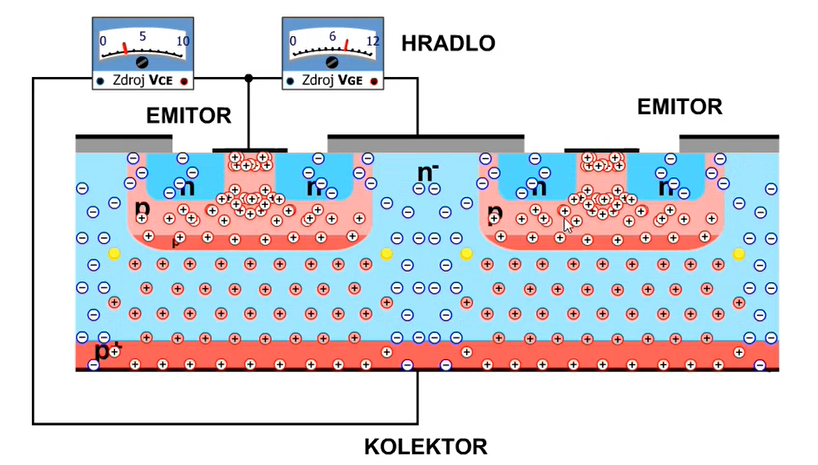
\includegraphics[width=12cm]{img/zzzzz.PNG}
    \caption{Náhľad na pôvodnú animáciu, vytvorené pomocou Adobe Flash}
    \label{Oldbutgold}
\end{figure}

To nám umožní, aby novovytvorené animácie boli dostupné študentom ešte veľa rokov. Súčasne, s rozvojom webových technológií, chceme týmto animáciám dať aj nové vlastnosti, akými sú responzivita, lepšia vizualizácia a lepšie ovládanie animácií.
\newline Okrem pôvodých animácií, ktoré boli vytvorené pre vyučovanie na \acrshort{FEI} \acrshort{STU}, existuje na internete iba jedno video  vo forme prezentácie, kde je animovaný princíp činnosti \acrshort{IGBT} tranzistora \cite{c29}. S tým videom študent však nemôže interagovať, ani vidieť ako sa menia vlastnosti \acrshort{IGBT} tranzistora, keď sa zmenia rôzne vstupné parametre. Na internete je ešte možné nájsť jednu simuláciu \acrshort{IGBT} tranzistora, ktorá nefunguje pravidelne a nedokáže vysvetliť študentom ako pracuje \acrshort{IGBT} \cite{c28}. Preto je naša práca významná, nielen pre študentov na \acrshort{FEI}, ale aj pre celú internetovú verejnosť.

\subsection{Popularizácia vedy a techniky}
Popularizácia vedy a techniky je komunikácia medzi členmi vedeckého spoločenstva a bežnými ľuďmi, občanmi, potenciálnymi konzumentmi vedeckých poznatkov. Tento druh vedeckej komunikácie má slúžiť aj ako marketing vedy, kde zrozumiteľné predstavenie produktov vedeckého bádania má jednak podporiť ich využiteľnosť a prínos pre bežný život ľudí, jednak podporiť chápanie oprávnenosti výdavkov na vedu a výskum. Zároveň sa predpokladá, že široká verejnosť je zdrojom potenciálnych mladých adeptov vedy.
\newline Podľa správy Eurobarometra z 21. júna 2010 takmer 80\% Európanov tvrdí, že sa zaujímajú o vedecké objavy a technologický vývoj. Vyše 70\% Európanov si myslí, že výskum financovaný zo zdrojov EÚ sa rozšíri, 57\% si myslí, že vedci by mali vynaložiť väčšie úsilie, čo sa týka šírenia informácií o svojej práci, a 66\% sa domnieva, že by vlády mali robiť viac pre to, aby vyvolali záujem mladých ľudí o vedecké otázky \cite{c14}. Pomocou interaktivitou a animáciami sa snažíme zvýšiť tieto percentá. Preto si spravíme analýzu na to, prečo sú animácie aj interaktivita výhodné, a takmer, v súčasnej dobe nutné pri vzdelávaní.

\subsubsection{Vzdelanie}
Ešte vo staroveku, detí sa učili hrou a objavovaním. Ten fakt stále platí aj v dnešnej dobe. V najmladších rokoch svojho života sa najviac naučíme, lebo sa stále hráme a objavujeme nové veci. Vo viacerých krajinách sveta, vzdelanie je nevyhnutnou súčasťou života ľudí a pomáha im dosiahnuť veľké veci. V súčasnosti používame rôzne techniky vzdelávania na zvýšenie efektívnosti a zniženie náročnosti učebného procesu. V 21. storočí infraštruktúra internetu neustále rastie; preto online vzdelávanie dostalo väčší priestor. Teda môžeme uzavrieť, že pre ľudí je  internet známe postredie, kde zvyčajne radi robia rôzne aktivity. Ďalšia výhoda online vzdelávacích materiálov je dosiahnuteľnosť. Študenti majú prístup k danému obsahu zo svojho počítača, tabletu, mobilného alebo podobného elektronického zariadenia.

\subsubsection{Interaktivita}
Existuje mnoho spôsobov, ako vytvoriť vzdelávací obsah. Vďaka interaktivite žiaci majú viaceré možnosti riadenia využitia študijného materiálu. Napríklad, s interaktívnymi animáciami majú možnosť upravovať parametre, meniť priebeh animácií, skákať dopredu alebo dozadu,  voliť si rôzne možnosti, atď. Zaradenie interaktivity do štúdia výrazne zvyšuje efektivitu štúdia. V roku 1969 Edgar Dale dokončil výskum o tom, ako si ľudia dokážu zapamätať najväčšie množstvo informácií. Všetci prítomní študenti si museli zapamätať  rovnaké informácie. Dale zdokumentoval výsledky a na ich podklade  vytvoril Kužeľ skúsenosti (Obrázok \ref{CE}). Interaktivitou dosiahneme priamu, účelovú skúsenosť, ktorá je na spodku kužeľa, kde je percento zapamätaných informácií  najvyššie \cite{c15}.

\begin{figure}[!htbp]
    \centering
    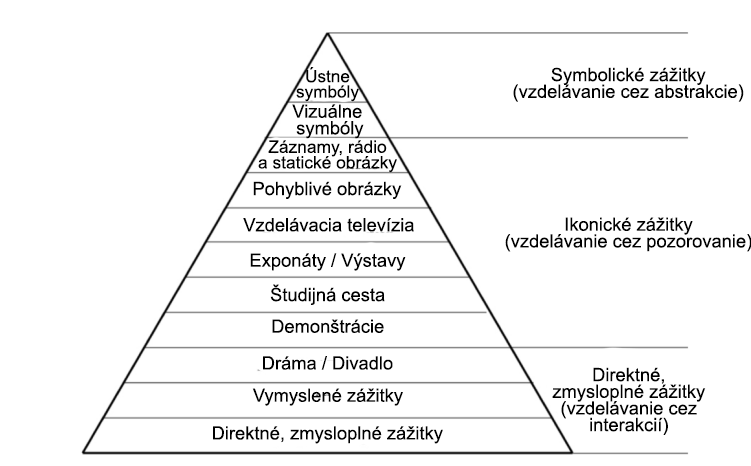
\includegraphics[width=12cm]{img/Cone-of-Experience.png}
    \caption{Kužeľ skúseností, ktorý predstavuje percento zapamätaných informácií daným spôsobom vzdelania \cite{c15}}
    \label{CE}
\end{figure}

\subsubsection{Animácia}
Aby sme vytvorili animáciu, najprv sa musia nakresliť jednotlivé obrázky. Ak zobrazíme tieto obrázky jeden po druhom veľmi rýchlo, vytvára sa ilúzia pohybu. V roku 1832 Joseph Plateau vytvoril fenakistoskop, ktorý zaviedol stroboskopický princíp modernej animácie \cite{c17}. V priebehu rokov ľudia experimentovali s rôznymi metódami simulácie pohybu. 
\newline Jednou z populárnych techník na vytváranie animácií je stop-motion. Prvým krokom je snímanie fotoaparátom skutočných objektov v počiatočnej polohe a potom po každej malej úprave sa znovu snímajú. Posledným krokom je  skladanie jednotlivých obrázkov pomocou špecifického softvéru na animovanie.
\newline Parameter \acrshort{FPS} - predstavuje počet snímok za sekundu a kvalitu animácií určuje práve ich počet. Ak sa snímková frekvencia zvyšuje, animácie budú plynulejšie. Pod 10-12 \acrshort{FPS} sa ešte stále vidia jednotlivé obrázky, pri frekvencii 12 až 24 snímok za sekundu by sme sa stále nemuseli cítiť príjemne. 24 \acrshort{FPS} FPS je najnižšia prijemná rýchlosť, pri ktorej ľudské oko dokáže vnímať pohyb, a 60 \acrshort{FPS} je teoreticky najväčšie obmedzenie, lebo nad tou frekvenciou väčšina ľudí nevidí rozdiel v kvalite animácií \cite{c16}.

\subsection{Raster vs. Vektor}
V tejto podkapitole porovnáme dva typy grafických možností, ktoré možno využiť v našej práci.
Vektorovú grafiku tvoria počítačové obrázky vytvorené pomocou sekvencie príkazov alebo matematických vzorcov, ktoré umiestňujú čiary a tvary do dvojrozmerného alebo trojrozmerného priestoru. Súbor vektorovej grafiky popisuje sériu bodov, ktoré sa majú spojiť a spoločne  vytvoriť nejaký objekt. Tieto súbory sa nazývajú aj geometrické súbory. Obrázky,  vytvorené pomocou nástrojov, akými sú Adobe Illustrator a CorelDRAW od Corelu sú zvyčajne súbory na prácu s vektorovými obrázkami \cite{c19} (Obrázok \ref{Vector}).

Keďže iba súbor matematických výpočtov musí byť uložený na vytvorenie obrazu, výstup vektorovej grafiky zaberá menší priestor v pamäti. Konverzia vektorového obrázku na rastrový obrázok je jednoduchá, pretože už máme matematické vzorce a nemusíme ich počítať. Prípony vektorového obrázku: .svg, .eps, .ai, .dxf atď.

\begin{figure}[!htbp]
    \centering
    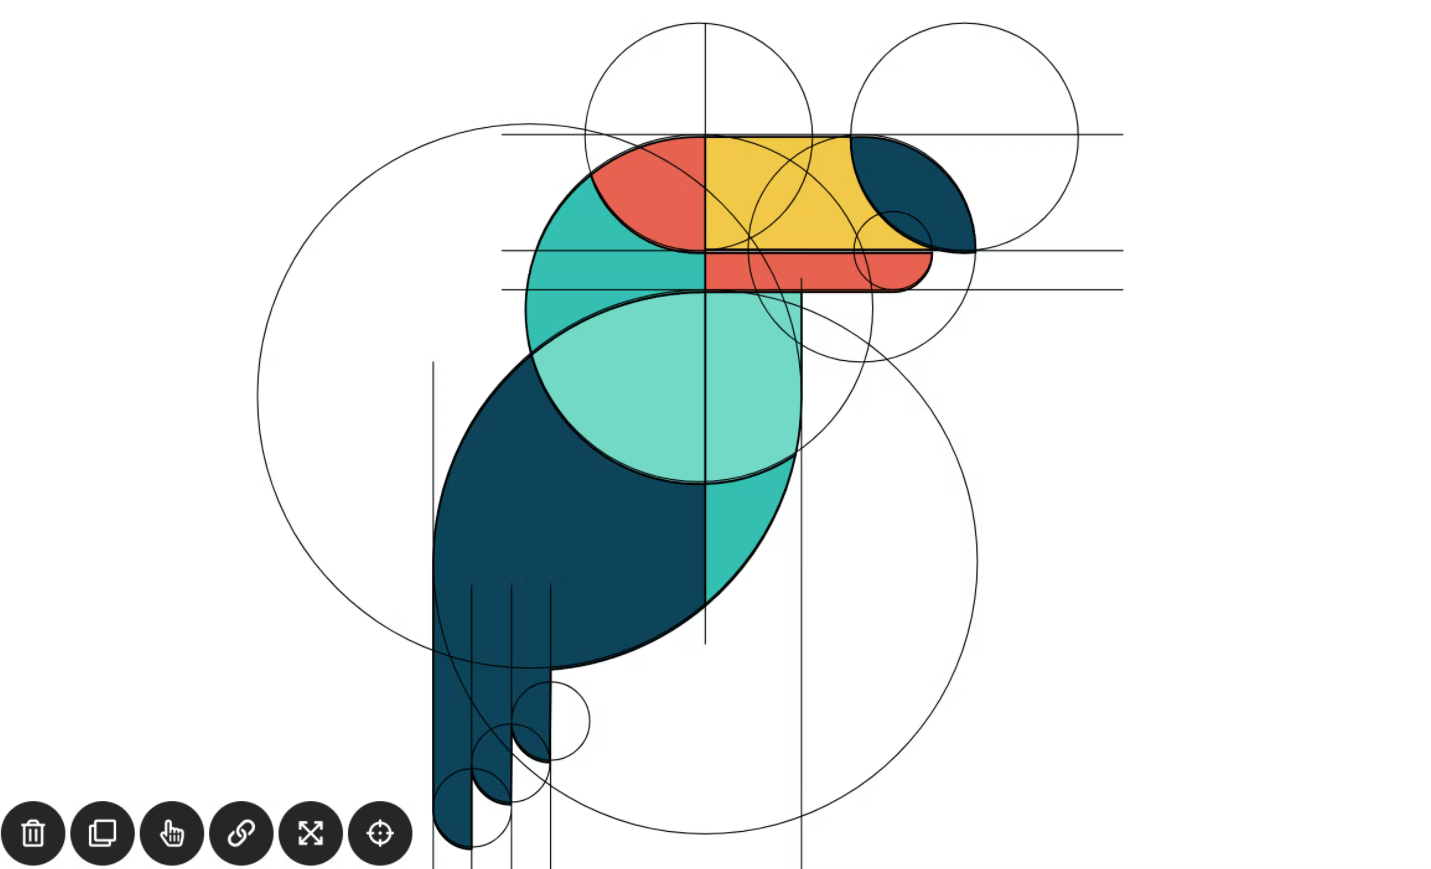
\includegraphics[width=12cm]{img/Vector.PNG}
    \caption{Vektorová grafika v editore \cite{c21}}
    \label{Vector}
\end{figure}

Rastrovú (bitmapovú) grafiku, tvoria digitálne obrázky, ktoré pozostávajú z malých obdĺž- nikových pixelov, ktoré sú usporiadané do mriežky alebo rastra súradníc \"x\" a \"y\"(zahŕňa aj súradnicu \"z\" v prípade 3D (trojrozmerný priestor)). Takým spôsobom sa tvorí obraz, lebo tie pixely sú zvyčajne zanedbateľné holým okom. Rastorovú grafiku často nazývame aj bitmapová grafika, pretože obsahuje informácie, ktoré sú namapované priamo do mriežky obrazovky \cite{c18}.

Veľké súbory môžu spomaliť rýchlosť načítania webovej stránky. Rastrová grafika je zvyčajne detailnejšia ako vektorová grafika. Jej nevýhody sa zjavujú pri zoomovaní, kedže v obraze založenom na pixeloch, množstvo údajov je konštantné a strate kvality sa nedá vyhnúť. Prípony rastrového obrázku: .bmp, .tif, .gif, jpg, .png atď.

\noindent Porovnanie týchto dvoch typov grafiky je možné vidieť na obrázku Obrazok \ref{VectorvsRaster}.

\begin{figure}[!htbp]
    \centering
    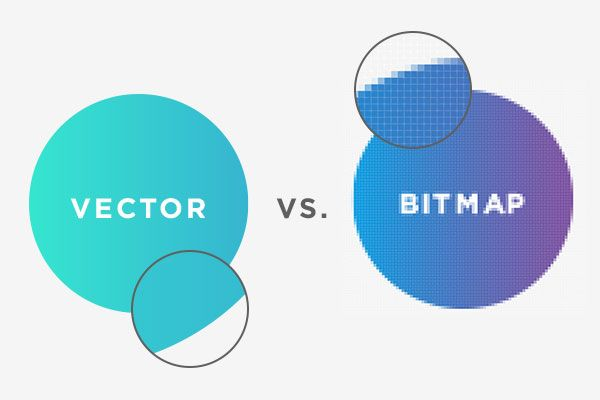
\includegraphics[width=12cm]{img/Vector vs Raster.jpeg}
    \caption{Vektorová grafika vs Rastrová grafika \cite{c20}}
    \label{VectorvsRaster}
\end{figure}

\newpage

\subsection{Analýza použitých softvérov} 
\noindent Pri voľbe softvéru na vytváranie animácií, dôležité je oboznámiť sa so softvérmi, ktoré sa na tento účel používajú, s ich výhodami, nevýhodami a dostupnosťou. Taktiež je vhodné spraviť analýzu programovacích knižníc, ktoré je možné na takéto účely použiť.

\subsubsection{HTML5} 
\noindent \acrshort{HTML} je štandardný značkovací jazyk, ktorý sa používa na vytváranie a modifikovanie webových stránok \cite{c2}. Je podporovaný všetkými známymi a aktuálnymi web prehliadačmi, a je najlepším softvérom na tvorbu webových stránok. Pomocou \acrshort{HTML5}, všetky stránky vizualizujú svoj obsah používateľom, prostredníctvom semantického značkovania. \acrshort{HTML} tvoria elementy, ktoré sú označené v tvare <>. Tie elementy potom tvoria štruktúru web stránky. Pretože \acrshort{HTML5} je veľmi perspektívny nástroj, rozhodli sme sa ho používať v našom projekte. HTML je dostupný všetkým a má elegantnú syntax, ktorá je dobre čitateľná. Podporuje rôzne multimédiá, akými sú audio a video súbory, má dobrú komunikáciu s prehliadačmi a rozsiahle vývojové prostredie. HTML poskytuje veľmi širokú škálu použitia, ako napríklad pri  animácii, web hrách, stránkach, serveroch a inom. Hlavnou nevýhodou je, že niektoré funkcie HTML5 nepracujú rovnako alebo vôbec na všetkých internetových prehliadačoch. Neaktuálne prehliadače, akým je Internet Explorer, nepodporujú HTML5. Taktiež, jediné prostredie, kde sa dá otestovať vlastný kód, je webový prehliadač a každú konzolu webového prehliadača je ťažko ovládať.

\subsubsection{CSS} 
\noindent \acrshort{CSS} (Cascading Style Sheets) je kaskádny štýl, ktorý slúži na formátovanie web stránky a pracuje v rámci s HTML5 elementmi, triedami, id a mení im rôzne vlastnosti -  farbu, font, veľkosť, tvar a polohu na stránke \cite{c3}. Vďaka tomu sa dostaneme k pekným dizajnom webovej stránky. Taktiež, CSS môže kontrolovať formát viacero webových stránok. Okrem toho, je možné animovať niektoré vlastností web stránok pomocou CSS, akými sú priechody a pohyby jednotlivých elementov. CSS je relatívne ľahké používať, ale hlavnou nevýhodou je, že jednotlivé CSS znázornenia nefungujú rovnako na každom prehliadači, preto je nevyhnutné podrobnejšie ich otestovať.

\subsubsection{JS}
\noindent \acrshort{JS} (JavaScript) je skriptovací jazyk pre web a pracuje v rámci s HTML5 \cite{c3}. JS nám umožňuje implementovať komplexné vlastností k webovým stránkam tak, že ovláda HTML elementy a ich CSS vlastnosti [16]. Má veľmi jednoduché používanie, jednoduchú syntax a môže vykonať veľa funkcií, akými sú e výpočet matematických funkcií, kreslenie, animovanie, riadenie webovej pamäti a iné. JavaScript je rýchly, má jednoduchú syntax a je ľahký na použitie. Hlavnou nevýhodou je, že nemá vytvorené prostredie na debagovanie. Preto hľadanie chýb v zložitom kóde je veľmi komplikované. JavaScript má predvolené funkcie pre animovanie, ale je oveľa výhodnejšie si zvoliť jednu alebo viac JS knižníc pre animovanie. JS knižnice nám ušetria čas, lebo už majú nakódované funkcie pre animovanie. Súčasne už majú nakódované vyhladené animácie a relatívne ľahko ich je  používať. Niektoré z najznámejších JS knižníc pre animovanie sú SVG.js, Anime.js, Gsap.js a JQuerry.

\noindent
\textbf{SVG.js} je klasická knižnica na kreslenie, animovanie a manipulovanie \acrshort{SVG} komponentov \cite{c5}. Táto knižnica má jednoduchú syntax a čitateľný kód. Ale nie je dobre okomentovaná, a má nečitateľný kód pri zložitých animáciách.

\noindent
\textbf{Anime.js} je modernejšia knižnica na animovanie objektov \cite{c6}. Táto knižnica má trochu zložitejšiu syntax, ale veľmi jednoducho sa pomocou anime.js animujú veľmi pekné a plynulé animácie. Táto knižnica je dobre okomentovaná a je čitateľná aj pri zložitých animáciách.

\noindent
\textbf{Gsap.js} je najužitočnejšia knižnica pre animovanie \cite{c7}. Knižnica je dobre okomentovaná, má jednoduchú syntax a môže zvládnuť najkomplexnejšie animácie. Na rozdiel od ostatných knižníc, ktoré sme tu spomenuli, Gsap.js má platenú licenciu.

\noindent
\textbf{JQuerry} je všeobecne najznámejšia a najpoužívanejšia knižnica pre všeobecné účely \cite{c8}. JQuerry je open-source knižnica, ktorá zjednodušuje JS syntax a \acrshort{DOM} (Document Object Model) manipulácie. Taktiež sa JQuerry môže použiť pre vytvorenie jednoduchých animácií. 

\subsection{Integrované vývojové prostredie}
Pri vytváraní nového programu pomáha použiť \acrshort{IDE} - Integrované vývojové prostredie, aby programátor ušetril čas a efektívne  písal kód. IDE zvyčajne obsahuje kompilátor, debugger a editor zdrojového kódu. K hlavným funkciám IDE patrí zvýraznenie syntaxe, čo pomáha programátorovi opraviť svoje chyby pred kompiláciou. Dôležitou funkciou je aj debugging; programátor má možnosť použiť body prerušenia, krokovať cez riadok alebo blok kódu, čo umožňuje jednoduchšie vyhľadávanie chyby.

\noindent \textbf{Visual Studio Code} je softvér na programovanie \cite{c9} HTML kódu a webového vývoju. Veľmi je populárny na vytváranie HTML stránok, CSS a JS skriptovanie. Vie rozoznať HTML, CSS a JS kód, čo pomáha autorovi pri automatickom dopĺňaní pri písaní kódu. Je to veľmi moderné prostredie na programovanie, ktoré sa stále aktualizuje, ale nemá automatické ošetrenie funkčnosti kódu, ako má IntelliJ. Visual Studio Code má veľa pluginov a rozšírení, ktoré môžu byť užitočné pri HTML programovaní, ako je SFTP rozšírenie.

\noindent 
\textbf {\acrshort{SFTP}} rozšírenie je bezpečný prevod súborov na webe \cite{c10}. Toto rozšírenie sa dá zadarmo stiahnuť cez Visual Studio Code. Funkciou tohto rozšírenia je, že číta .json súbor, v ktorom môžeme zadať informácie o webovej stránky, na ktorej pracujeme. Prvýkrát keď je prečítaný tento súbor, SFTP vytvorí webovú stránku na zadanom serveri, vytvorí zadanú web adresu, a všetky naše zmeny v kóde budú automaticky aktualizované na sieti. Klasické riešenie vytvorenia stránky a aktualizovania zmeny kódu na stránke sa koná pomocou nástroja \acrshort{WinSCP}. 

\noindent
\textbf {\acrshort {WinSCP}} je open-source \acrshort{SFTP} klient pre Windows \cite{c11}. Jeho hlavnou funkciou je prevod súborov medzi lokálnym a diaľkovým počítačom, akým je server, na ktorom sa nachádzajú web adresy.  Užitočné je používať ho. V prípade, že sa programátorom nepodarí všetky súbory previesť cez Visual Studio Code, tak sa to dá urobiť manuálne cez WinSCP.

\subsection{Tranzistor IGBT}
\noindent \acrshort{IGBT} (Insulated Gate Bipolar Transistor) je výkonový tranzistor s izolovaným hradlom. Má dôležitú úlohu v elektrotechnike ako spínač, má rozsiahle použitie (ako napríklad v oblasti elektromobility, v energetike atď) a predstavuje krok do budúcností elektrotechnických výkonových zariadení. Vznikol spojením bipolárneho tranzistora - PNP na výstupe a unipolárneho tranzistora \acrshort{MOSFET} (N kanálový \acrshort{MOSFET}) na vstupe.

Schematickú značku \acrshort{IGBT} môžeme vidieť na obrazku Obrázok \ref{IGBTScheme}. Táto štruktúra umožňuje, aby tranzistor \acrshort{IGBT} bol ovládaný napätím pripojeným medzi hradlom a emitorom, a keďže \acrshort{IGBT} je kombinácia bipolárneho tranzistoru (\acrshort{BT}) a unipolárneho tranzistoru, cez časť, ktorú tvorí BT, preteká oveľa väčší prúd ako v prípade \acrshort{MOSFET} \cite{c22}.

\begin{figure}[!htbp]
    \centering
    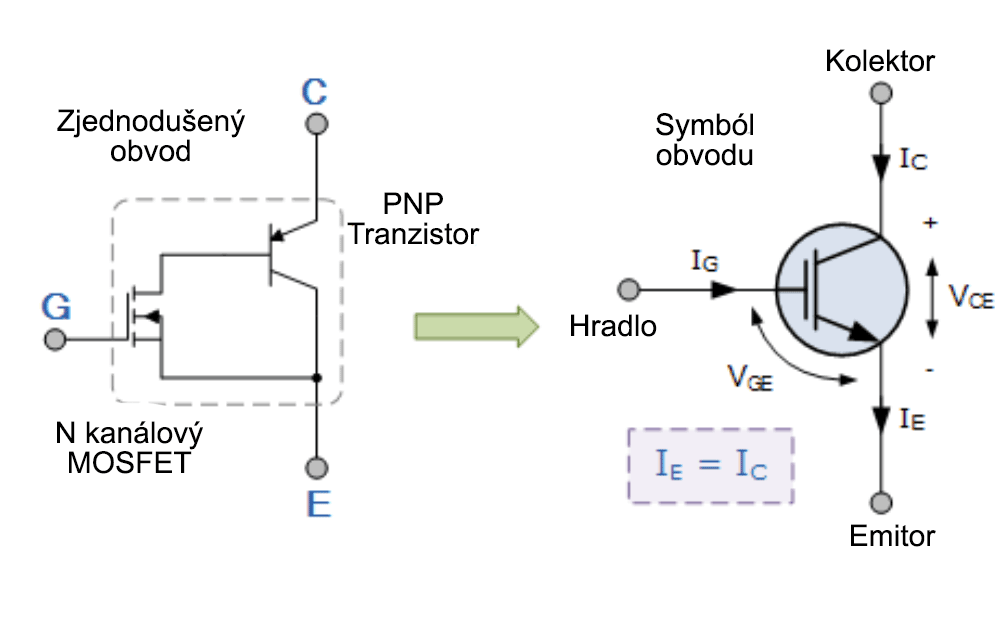
\includegraphics[width=12cm]{img/igbtscheme.PNG}
    \caption{N kanálový IGBT tranzistor, značky a náhradná chéma \cite{c22}}
    \label{IGBTScheme}
\end{figure}

\subsubsection{Princíp činnosti}
\noindent Na obrázku Obrázok \ref{IGBT} je zobrazená vnútorná štruktúra \acrshort{IGBT} tranzistora, ktorá sa podobá na \acrshort{MOSFET}. Avšak substrát N$^+$ je nahradený vrstvou s dopáciou P$^+$. Táto vrstva tvorí základ štruktúry bipolárneho tranzistora \acrshort{PNP} (Positive-Negative-Positive priechod). Z toho vyplýva, že \acrshort{IGBT} má na vstupe podobné vlastnosti ako \acrshort{MOSFET} - je riadený elektrickým poľom, a na výstupe má podobné vlastnosti ako bipolárny tranzistor. To znamená, že zabezpečuje vedenie vysokého prúdu pokiaľ je schopný kontrolovať intenzitu elektrického poľa.

\begin{figure}[!htbp]
    \centering
    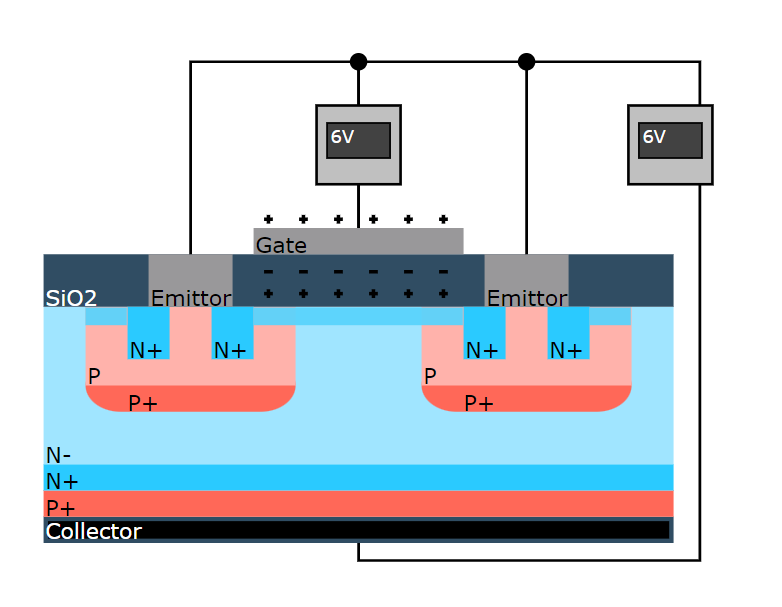
\includegraphics[width=12cm]{img/igbt.PNG}
    \caption{Grafické znázornenie vnútornej štrutkúry IGBT}
    \label{IGBT}
\end{figure}

Tranzistory sú tvorené z polovodičových materiálov, v tomto prípade sa to jedná o kremík. Každý atóm kremíka je spojený so štyrmi susednými atómami kremíka. Atóm kremíka má štyri valenčné elektróny a zdieľa každý tento elektrón s jedným susedom v kryštalickej mriežke. Čistý kremík je prakticky nevodivý, preto aby sme zvýšili jeho vodivosť pridávame prímesy. Poznáme dva typy prímesov. P-typ - je prímes cudzieho materiálu z tretej skupiny (napr. Bór), ktorý má iba tri elektróny vo valenčnej vrstve. Vďaka tomu, že im chýba jeden elektrón, vznikajú nové miesta bez elektrónov, ktoré nazývame diery. N-typ - je prímes materiálu z piatej skupiny, ktorý má 5 elektrónov vo svojej valenčnej vrstve, ktoré dodávajú voľný elektrón do systému .Správajú sa ako donori. Tieto elektróny sa môžu voľne pohybovať v našom systéme. IGBT pozostáva z niekoľkých vrstiev, ktoré sú P-typu alebo N-typu. Po spojení P a N vrstvy vzniká PN priechod. V tejto oblasti PN priechodu je vrstva ochudobnená o majoritné nosiče náboja a elektróny v N-type difundujú do P časti. Tento pohyb nastáva vďaka difúzii nosičov, a táto difúzia je dôsledkom gradientu koncentrácie jednotlivých nosičov náboja. Dôsledkom toho bude, že P časť bude mať mierne záporne nabitú vrstvu a N časť bude mať mierne kladne nabitú vrstvu na rozhraní. Vďaka tomu vzniká vnútorné elektrické pole, ktoré zastaví ďalší pohyb elektrónov z jednej k druhej vrstve.

Aby sme umožnili elektrónom pohyb cez kanál tranzistora, musíme pripojiť vhodne polarizované napätie, ktoré spôsobí presun elektrónov do P časti. Vzniká veľký rekombinačný prúd, lebo veľa elektrónov zaplní diery v P časti. Nazývame to priepustno polarizovaný priechod. Ak pripojíme záverne polarizované napätie, tak PN priechod bude záverne polazirovaný. Tento priechod vplýva na zväčšovanie ochudobnenej oblasti, ktorá zastaví tok elektrónov. Pripojením napätia na izolované hradlo, SiO$_2$, pôsobí ako izolačná vrstva, bude záporne nabitý na strane hradla. Z druhej strany, bude izolačná vrstva nabytá kladne. Kladné nabitie pritiahne elektróny v P časti, a to vytvorí inverznú vrstvu, ktorú nazývame kanál. Táto vrstva sa  zväčšuje, v závislosti od veľkosti napätia, ktoré pripojíme medzi hradlo a emitor. Tento kanál vytvorí elektrónom cestu a elektróny sa budú môcť pohybovať cez priepustne polarizovaný priechod \cite{c25}. 

Elektrický prúd najprv rastie so zvyšovaním  napätia na kolektore, ale pri vyššom napätí dôjde k zaškrteniu kanála (Obrázok \ref{IGBTSGraph}). Tento bod sa nazýva pinch-off. Vďaka tomu, naším kanálom už tečie konštantný prúd, bez ohľadu na pripojené napätie \cite{c24}.

\begin{figure}[!htbp]
    \centering
    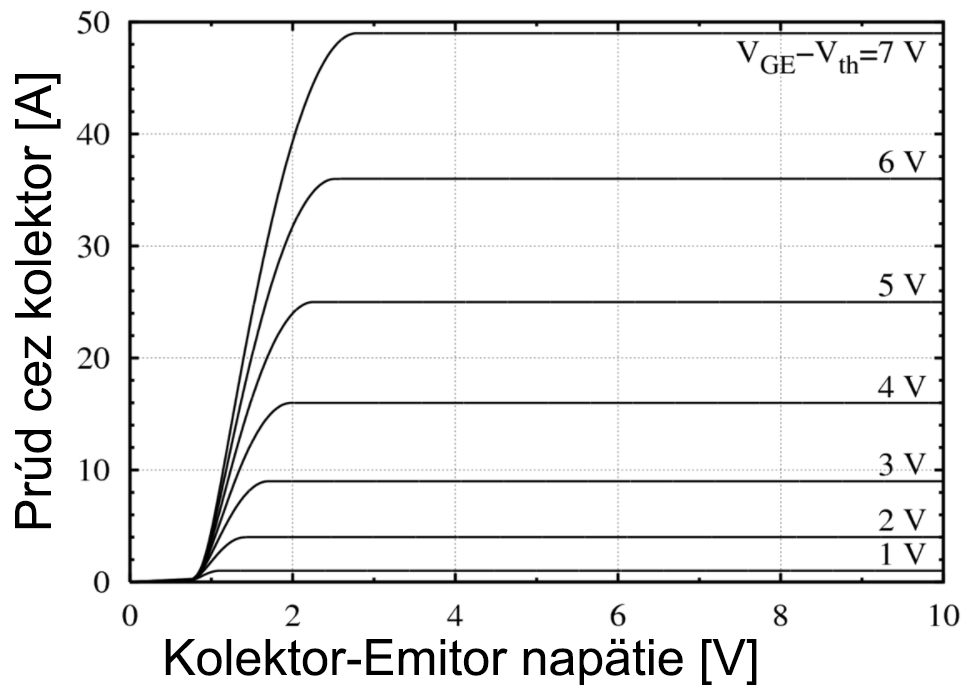
\includegraphics[width=12cm]{img/igbtgraph.PNG}
    \caption{Volt-ampérové charakteristiky IGBT \cite{c24}}
    \label{IGBTSGraph}
\end{figure}

\newpage

\subsubsection{Aplikácie}
V roku 2022, \acrshort{IGBT} je druhý najvyužívanejší tranzistor vo svete, po \acrshort{MOSFET} tranzistoroch. Zodpovedá 27\% výkonných tranzistorov na trhu, na vstupe RF (Radio frequency) zosilňovača (11\%). \acrshort{IGBT} sa používa rovnako ako bipolárny tranzistor; na zosilňovanie a spínanie signálov a realizáciu logických funkcií. V súčasnosti je najčastejšie používaný na spínanie veľkých prúdov nad 10 A pri napätiach nad 600 V (graf použitia na základe napätia a prúdu na obrázku Obrázok \ref{IGBTApp}). Vývoj tranzistora \acrshort{IGBT} podnietila snaha o spojenie výhod bipolárnych tranzistorov a tranzistorov \acrshort{MOSFET} vo výkonových aplikáciách. IGBT má široký rozsah použití - v priemyselnej technológií, každodennej elektronike, energetickom sektore, vesmírnych zariadeniach ako aj v nových prostriedkoch dopravy \cite{c23}.

\begin{figure}[!htbp]
    \centering
    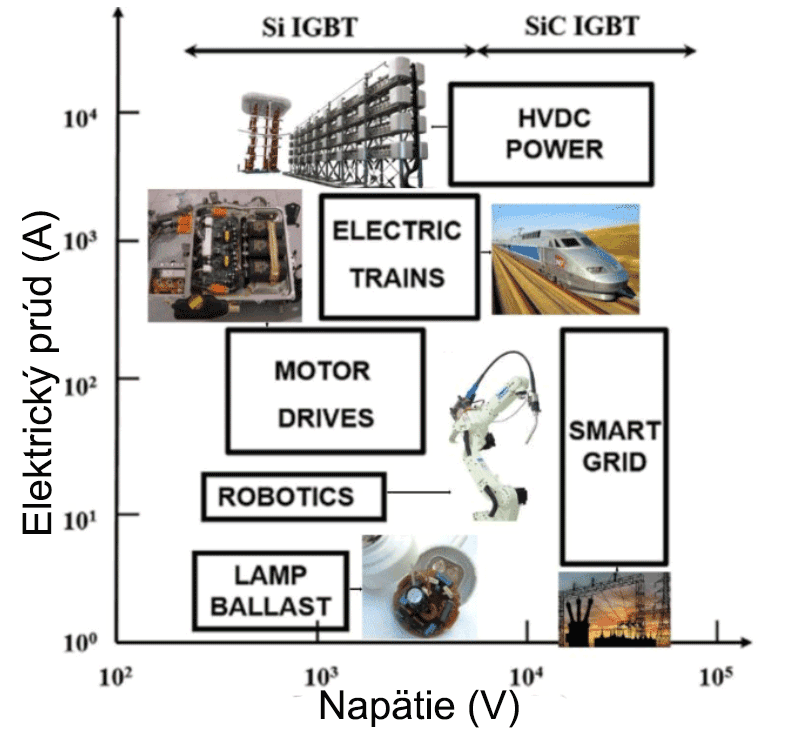
\includegraphics[width=11cm]{img/igbtapp.PNG}
    \caption{Graf použitia IGBT na základe napätia a prúdu \cite{c23}}
    \label{IGBTApp}
\end{figure}

\newpage

\subsection{Záver analýzy}
Vysvetlili sme si význam interaktívnych vzdelávacích animácií a následne sme porovnávali rastrovú grafiku s vektorovou grafikou. Ďalej sme si posvietili na  možnosti softvéru, vzory dizajnu, technológie a koncepty pre našu animáciu. Rozhodli sme sa použiť HTML a CSS pre návrh a tvorbu webových stránok, a kódovať v JavaScript programovacom jazyku. Implementujeme grafiku a animácie pomocou knižnice SVG.js. Na vývoj použijeme IDE Visual Studio Code. Rôzne interaktívne elementy budú implementované, aby zvýšili efektivitu vzdelávania. Namiesto vytvárania iba jednej animácie, rozhodli sme sa zobraziť viacero paralelných animácií, každá z nich pristupuje k inému problému. Naša aplikácia vysvetlí princíp činnosti \acrshort{IGBT} tranzistora s využitím nového prístupu webových technológií, čo poskytuje najefektívnejšie riešenie  študentom na rýchle pochopenie problematiky.

\section{Opis riešenia}
V tejto kapitole sa budeme venovať príprave na splnenie všetkých požiadaviek pri  vytvorení stránky, animácií a interaktivity nášho projektu. Prichystáme si návrh layoutu našej webovej stránky pre desktopy a mobilné zariadenia. Pomocou \acrshort{UML} diagramu tried, znázorníme návrh vlastností a metód našej stránky. Potom si vysvetlíme, ako sme implementovali naše  animácie a interaktívne vlastnosti, a na konci si overíme naše riešenie.

\subsection{Špecifikácia problému}
Naša animácia musí presne opísať, ako funguje \acrshort{IGBT} tranzistor. Pretože princíp činnosti \acrshort{IGBT} tranzistora je zložitý, vytvoríme model, ktorý študentom stačí na pochopenie fyzikálneho deja v \acrshort{IGBT} tranzistore. Dbáme aj na to, aby sme nevynechali dôležité detaily. Na základe analýzy použijeme \acrshort{SVG}na vytvorenie samotnej animácie a grafiky \acrshort{IGBT} tranzistora. Layout webovej stránky musí byť prispôsobené používateľovi. Na stránke musíme používať slovenský a anglický jazyk, aby sme našu stránku prispôsobili aj študentom, ktorým slovenčinu neovládajú až tak dobre.  Animácia musí vysvetliť tieto udalosti:  princíp činnosti \acrshort{IGBT} tranzistora, volt-amperové charakteristiky, zmenu animácie po výmene napätia na kolektore alebo na hradle. Používateľ musí mať možnosti interagovať s animáciou a ovplyvňovať ju, všetky vyššie uvedené udalosti musia v prípade potreby reagovať na interakciu a tiež musia byť navzájom synchronizované.

\subsection{Návrh riešenia}
Pre tvorbu interaktívnej animácie sa nám ako najlepšie ukázalo riešenie v štandardnom značkovacom jazyku HTML5. Taktiež budeme využívať funkčnosti CSS aj JavaScriptu, ktoré pracujú v rámci s HTML5. Tiež sme sa rozhodli, že jednotlivé animácie a obsahy umiestnime do podstránok, a rozdelíme ich do jednotlivých kapitol. Týmto riešením sa dosiahne lepšia prehľadnosť a jednoduchosť aplikácie. Pre testovanie funkčnosti stránky využijeme \acrshort{FEI} cloud webový server v rámci s Google webovým prehliadačom, aby sme otestovali jednotlivé funkcie stránky, ktoré  nemožno otestovať na lokálnom serveri.

\subsubsection{Dizajn}
Dizajn je dôležitou súčasťou procesu vývoja aplikácie. Ak už máme základnú predstavu, ako by mal náš projekt vyzerať, ďalším krokom by mala byť vizualizácia konceptu. Kreslenie náčrtu nám pomáha urobiť vizualizáciu nápadu na vytvorenie našej stránky. Vytvorenie UML alebo iného modelovacieho diagramu uľahčuje programovanie štruktúry stránky. Plánovanie dopredu nám pomáha, aby sa náš kód dal čím lepšie udržiavať a rozširovať. Farebná škála našej stránky je inšpirovaná farebnou škálou stránky www.w3schools.com.

Takisto treba rozmýšľať aj o vizuálnom dizajne  našej stránky. Chceme aby naša  stránka mala pekný vzhľad na každom zariadení. Dobre je plánovať, aby všetky elementy, ktoré sú viditeľné používateľovi, pri načítaní stránky na desktope boli viditeľné aj používateľovi na mobilnom zariadení. Dobrým nápadom ako toto riešiť je mriežkový (gridový) dispej a PWA (Progressive Web App).

Znázornenie elementov v mriežke nám uľahčuje kontrolu ukážky elementov na rôznych zariadeniach. Napríklad, chceli by sme aby naše elementy boli poskladané v mriežke $2\times 3$ (dva rady a tri stĺpce) pri väčších obrazovkách. Pri menších obrazovkách, chceme postupne zmeniť ten grid na $3\times 2$, aj konečne na $6\times 1$ pre mobilné zariadenia. Obrázok 9 zobrazuje ukážku, ako by to malo vyzerať.

\begin{figure}[!htbp]
    \centering
    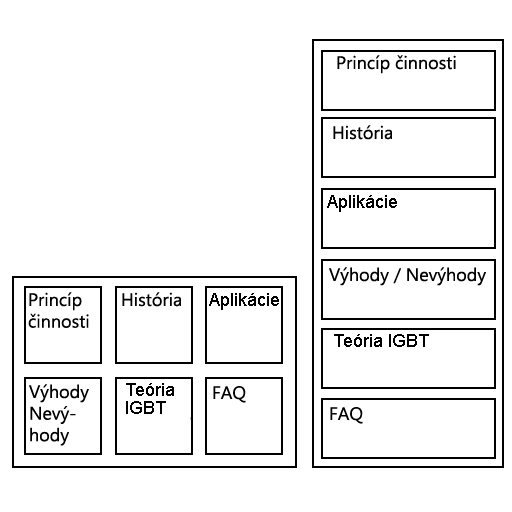
\includegraphics[width=12cm]{img/Layout.png}
    \caption{Layout na veľkej obrazovke (vľavo) a layout na malej obrazovke (vpravo)}
    \label{Layout}
\end{figure}

\acrshort{PWA} Progressive Web App je webová stránka, ktorá vyzerá a správa sa, ako keby išlo o mobilnú aplikáciu. PWA sú vytvorené tak, aby využívali funkcie mobilného zariadenia bez toho, aby konečný používateľ musel navštíviť obchod s aplikáciami, kúpiť a stiahnuť softvér lokálne. PWA sa nemôže otestovať na lokálnom serveri, preto je potrebné vhodné umiestnenie na webovom serveri. Vhodné nastavenie PWA sa otestuje pomocou Lighthouse webowého rozšírenia. Lighthouse rozšírenie nám automaticky otestuje, či naša webstránka spĺňa všetky podmienky PWA (Obrázok \ref{pwa}) \cite{c26}.

\begin{figure}[!htbp]
    \centering
    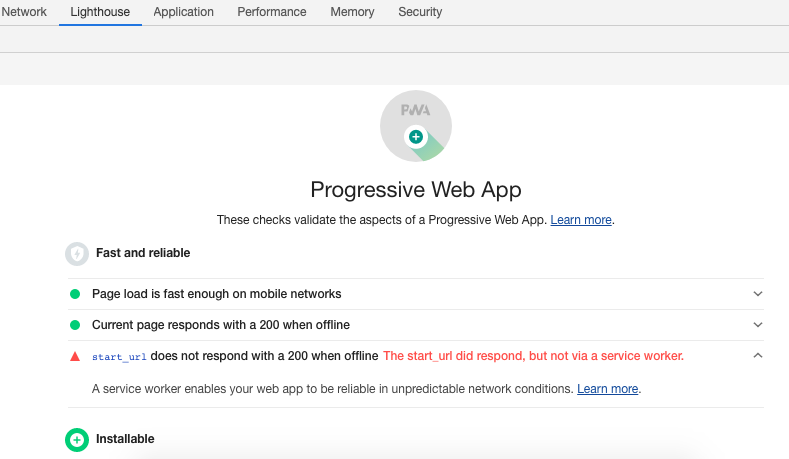
\includegraphics[width=12cm]{img/PWA.png}
    \caption{Ukážka testu Progressive Web Appu  \cite{c30}}
    \label{pwa}
\end{figure}

\subsubsection{UML Case diagramy}
Jedným z najpopulárnejších spôsobov návrhu a modelovania je použitie UML Case diagra- mov. V UML Case diagrame špecifikujeme vzťahy medzi triedami. UML Case diagramy sa dajú vytvoriť rôznymi spôsobmi. My sme využili app.diagrams.net na tvorbu diagramov. Obrázok \ref{UMLMain} zobrazuje návrh našej hlavnej stránky. 

\begin{figure}[!htbp]
    \centering
    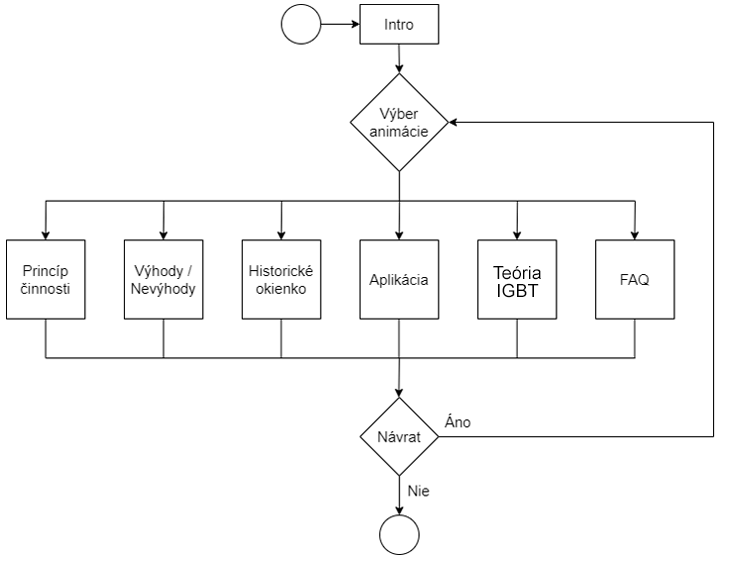
\includegraphics[width=12cm]{img/UMLMain.png}
    \caption{Návrh úvodnej stránky}
    \label{UMLMain}
\end{figure}

Ako prvú animáciu na webstránke budeme mať intro, ktoré bude mať za úlohu zaujať používateľa a prilákať ho k téme \acrshort{IGBT} tranzistory.  V strede hlavnej stránky sa nachádza tlačidlo, ktoré otvorí a pustí video,  predstavujúce úvod k našej web stránke. Video predstavuje krátku prezentáciu, ktorá popisuje základné a zaujímavé vlastnosti \acrshort{IGBT}, aby používateľ mal predstavu, o čom sa vlastne má naučiť. Používateľ sa potom môže na podklade vlastnej vôle prepnúť na hociktorú podstránku. Každá podstránka má svoj význam. Na podstránke "Princíp činnosti"\ sa nachádza hlavná animácia s interaktívnymi elementmi, spolu s grafom volt-ampérových charakteristík. Na podstránke "História"\ sa nachádza mapa vývoja \acrshort{IGBT} tranzistora, spolu so slajderom, ktorý znázorňuje grafickú ukážku jednotlivého modelu \acrshort{IGBT} tranzistora. Na podstránke Aplikácia"\ sa nachádza niekoľko  príkladov použitia \acrshort{IGBT} tranzistora, aby používateľ pochopil, aký veľký rozsah použití má \acrshort{IGBT} tranzistor. Na podstránke "Výhody/Nevýhody"\ sa nachádza jednoduchý zoznam; aké sú výhody a nevýhody \acrshort{IGBT} vo reálnom svete. Na podstránke "Teória IGBT"\ sa nachádza postupné vysvetlenie čo prebieha v \acrshort{IGBT} tranzistore na fyzickej úrovni, ako funguje, aj prečo sa \acrshort{IGBT} nazýva Bipolárny tranzistor s izolovaným hradlom. Nakoniec, podstránka "FAQ"\ bude obsahovať často kladené otázky (Frequently Asked Questions). Aby používateľ nebol zmätený, každé prepájanie na hlavnú stránku má zoznam vlastnej podstránky. Používateľ bude v každom prípade vedieť, kde má čo hľadať.

\subsubsection{Štandardizácia animácie}
Na eLearn Central je k dispozícii množstvo animácií a mnohé z nich majú podobnú tému. Ak študenti navštívia túto stránku, zvyčajne otvoria niekoľko animácií, ktoré popisujú podobné procesy. Tieto animácie sa riadia rovnakými princípmi, takže študent sa nemôže zmýliť. Chceme pridať našu animáciu do existujúcej kolekcie na eLearn Centrale, a to si vyžaduje definovanie farieb, používaných pre našu animáciu. Farby, ktoré sme definovali, sú uvedené tabuľke Tabuľka \ref{Farby}. Snažíme sa tiež dodržať rovnakú veľkosť a tvary jednotlivých objektov.

\begin{table}[!htbp]
\caption{Štandardné farby pre využitie v animácií}
\label{Farby}
\begin{center}
\begin{tabular}{ |c|c|c|c| } 
\hline
Meno & Farba výplne & Farba čiary & Symbol\\ \hline
Majoritný elektrón & \#FFFFFF & \#333399 & \#000000 \\ \hline
Majoritná diera & \#FFFFFF & \#FF0000 & \#000000 \\ \hline
Minoritný elektrón & \#37FFFF & \#333399 & \#000000 \\ \hline
Minoritná diera & \#FF9999 & \#FF0000 & \#000000 \\ \hline
'P' oblasť & \#FDACAC & \#FF0000 & - \\ \hline
'N' oblasť & \#CCECFF & \#0000FF & - \\ \hline
Ochudobnená oblasť & \#94FE70 & - & - \\ \hline
\end{tabular}
\end{center}
\end{table}

\subsection{Implementácia}
Teraz opíšeme proces, ktorým všetky naše návrhy a nápady implementujeme do nášho zadania.

\subsubsection{Tvorba webstránky}
Najprv si vytvoríme webovú stránku pomocou HTML5 štandardu. V tomto štandarde vytvoríme všetky potrebné elementy pre úspešnú validáciu. V tomto štandarde dva tagy: <!DOCTYPE html> a <html>. Potom, každý HTML súbor musí mať <head> tag, ktorý uschováva informácie o stránke (backend) a <body> tag, ktorý bude mať obsah našej stránky (frontend). Každá platná stránka musí mať meno, nuž musíme vložiť tag <title>. HTML5 si vyžaduje tag <meta charset = ütf-8», ktorý zabezpečuje využívanie neanglických znakov (akými sú dĺžne a mäkčene). Teraz musíme nahrať našu stránku na web. Na to využijeme SFTP rozšírenie, ktoré sa spojí so zadaným serverom a po zachovaní nášho kódu automaticky  aktualizuje našu stránku. Taktiež sa odporúča využívanie kaskadného štýlu pre dizajn (<link rel = "stylesheet"href = "css/style.css») a JavaScript pre ovplyvnenie  HTML elementov (<script src="js/script.js»</script>). Potom sme si pomocou HTML a CSS vytvorili štruktúru a vzhľad našich stránok pomocou rôznych elementov, tried a id, ktorým sme pridali rôzne vlastnosti, akými sú farba pozadia, veľkosť, dĺžka, umiestenie a iné.

\subsubsection{Jednoduchý úvod do JavaScriptu}
Prvá vec, ktorú si programátor uvedomí keď začína pracovať s JavaScriptom je tá, že JavaScript nepoužíva tradičné typy premenných (int, float, char...), ale má iba 3 typy premenných: const, var a let. Každý typ dokáže umiestniť akýkoľvek  typ premennej, dokonca aj zložité objekty. Const je konštantná premenná, čo znamená, že jej hodnotu priradíme hneď po deklarácií  a jej hodnotu nesmieme ďalej meniť. Var a let fungujú podobne. Oba typy povoľujú zmenu hodnoty premennej, avšak let nepovolí redefinovanie premennej (premenná s rovnakým menom ako meno premennej let sa nesmie znovu definovať). Funkcia console.log() slúži na výpis premenných. Táto funkcia je rovnako schopná vypísať aj najzložitejšie hodnoty premenných (Obrázok \ref{Log}). JS je schopný rozoznať koniec príkazu, takže nie je nutné využívať ; pre koniec príkazu ako je to v tradičných programovacích jazykoch povinné, ale takisto, nie je nutné používať odseky na zhrnutie kódu  funkcie, ani využívať nový riadok ako formu konca príkazu ako je to v programovacom jazyku Python. Hlavnou funkčnosťou JS je ovládanie HTML elementmi. JS je schopný vytvárať aj volať HTML elementy pomocou document funkcie. Najčastejšie sa stretneme s príkazom document.getElementById("id"), ktorý vráti element so zadaným idečkom, ktoré pripravíme na ovládanie. Obrázok \ref{alg0} zobrazuje zmenu rôznych html a css vlastností daného elementu. InnerHTML a TextContent funkcie ovládajú textom, ktorý sa nachádza v danom elemente a funkcia  style ovláda zadanú css vlastnosť elementu (akými sú veľkosť fontu, viditeľnosť, farba pozadia a rôzne).

\begin{figure}[!htbp]
    \centering
    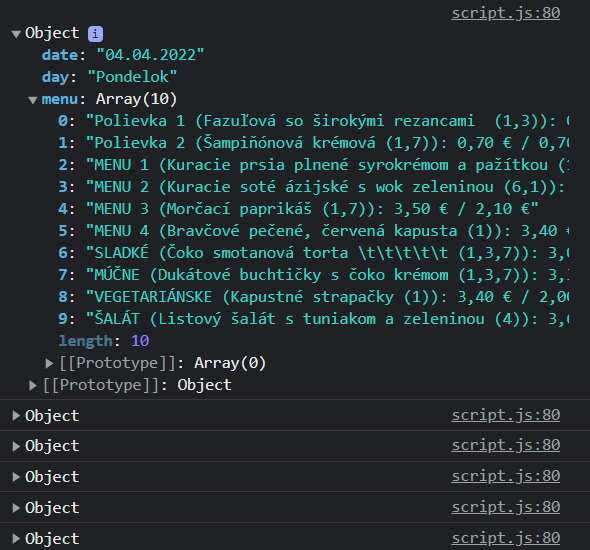
\includegraphics[width=10cm]{img/y.PNG}
    \caption{Ukážka konzolového výstupu zložitého objektu}
    \label{Log}
\end{figure}

\newcommand\tab[1][1cm]{\hspace*{#1}}

\begin{figure}[!htbp]
    \centering
    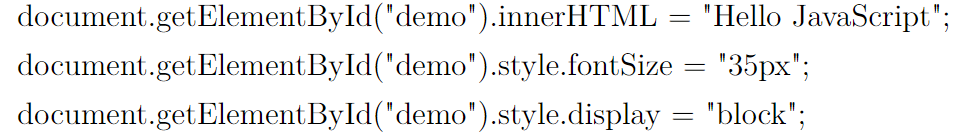
\includegraphics[width=15cm]{img/alg0.PNG}
    \caption{Ukážka ovládaní HTML elementov pomocou JavaScriptu}
    \label{alg0}
\end{figure}

\newpage

\subsubsection{Kreslenie a animácia IGBT}
\noindent Na kreslenie využívame svg.js knižnicu. Knižnicu je potrebné buď  prebrať a lokálne  ju referencovať, alebo je potrebné referencovať jej webový odkaz (odporúčaná je prvá možnosť). Týmto spôsobom môžeme využívať funkcie knižnice svg.js. Táto knižnica je schopná kresliť vektorové objekty, čo znamená, že nebudú zaberať veľa priestoru na našej stránke. Najprv vytvoríme kanvas, v ktorom budeme kresliť. Tento kanvas sme schopní ovplyvniť. Ďalej môžeme kresliť rôzne objekty, hlavne sú nám potrebné obdĺžniky, čiary a kruhy. Takisto sa môžu  na kanvas vkladať texty a obrázky. Týmto objektom môžeme okamžite meniť vlastnosti, akými sú ich poloha, veľkosť, transparentnosť a farba. Syntax svg.js knižnice je jednoduchá (Obrázok \ref{alg1}). Treba definovať kanvas. Zvolíme si objekt a potrebujeme mu zadať x a y polohu a jeho veľkosť v pixeloch. V prípade čiarok, potrebné je zadefinovať aspoň dve x a y súradnice v formáte (x,y x1,y1...). V prípade textu, treba vložiť string a umiestniť ho na kanvas.

\begin{figure}[!htbp]
    \centering
    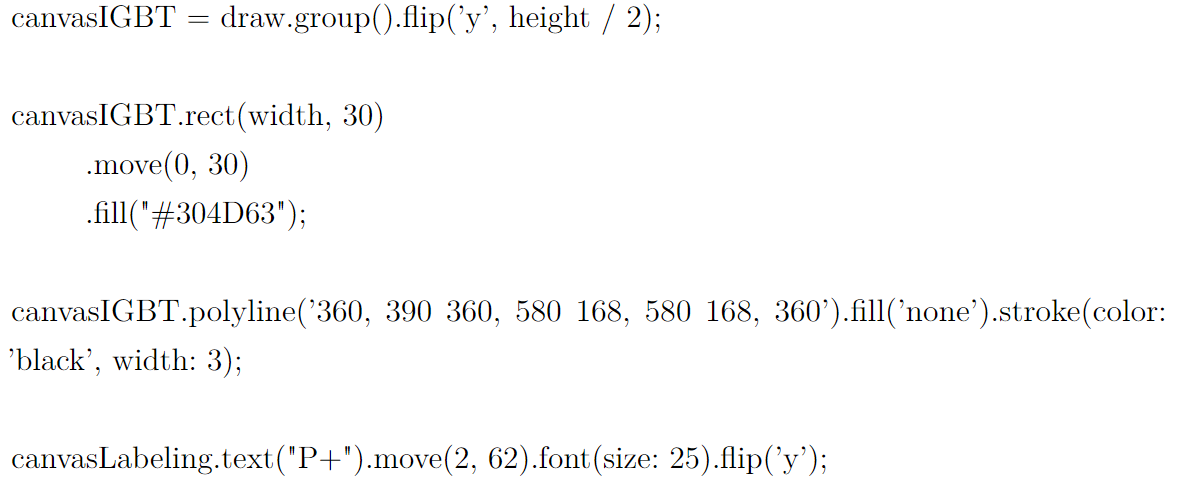
\includegraphics[width=15cm]{img/alg1.PNG}
    \caption{Ukážka príkazov pre použitie kanvasu}
    \label{alg1}
\end{figure}

Užitočné je robiť skupiny objektov, ktoré sa budú správať ako jeden prvok, aby sme potom mohli ovplyvňovať vlastnosti celého prvku. Napríklad, všetky prvky,  tvoriace grafické znázornenie \acrshort{IGBT} tranzistora, je vhodné zaradiť do skupín, aby sme mohli prípadne meniť  veľkosť celého tranzistora iba jedným príkazom.

Keď vhodne vytvoríme a umiestnime objekty, ktoré sme sa naučili vytvárať, naša výsledná grafika je znázornená na obrázku Obrázok \ref{IGBT2}.

\begin{figure}[!htbp]
    \centering
    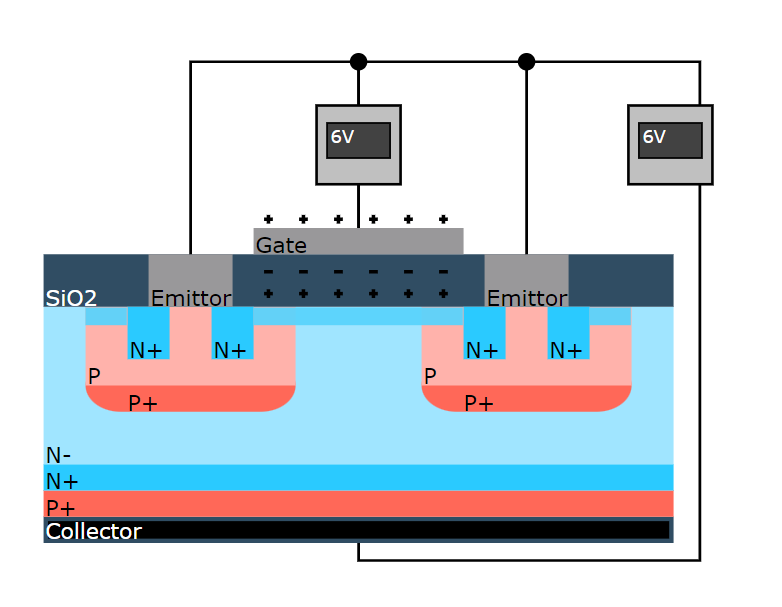
\includegraphics[width=12cm]{img/igbt.PNG}
    \caption{Vytvorený IGBT objekt}
    \label{IGBT2}
\end{figure}

Existuje ešte jeden vhodný spôsob na zhrnutie vytvorených \acrshort{SVG}objektov do skupín. Urobíme to tak,  že ich vložíme do poľa. Týmto spôsobom sa dajú zavolať funkcie, ktoré vytvoria skupiny objektov a uložia ich do poľa. Takto nemusíme vytvárať veľké množstvo premenných, ktoré predstavujú skupiny, ale stačí iba zavolať pole so vhodným indexom (Algoritmus \ref{alg2}) na ovplyvnenie žiadaného prvku. Pretože takéto prvky chceme využiť v animácii, vhodne sme si ich presunuli mimo obrazovky (stačí zadať záporný parameter x alebo y súradnici), aby sa objavili iba keď ich chceme znázorniť.

\begin{algorithm}
\begin{algorithmic}

\STATE function drawElectron(draw)\{
\STATE \tab let electron = draw.group().flip('y', height / 2);
\STATE \tab electron.clear();
\STATE \tab electron.circle(20).fill("\#333399");
\STATE \tab electron.circle(14).fill("white").move(3, 3);
\STATE \tab electron.line(5, 10, 15, 10).stroke({ color: "black", width: 4});
\STATE \tab return electron;
\STATE\}
\STATE
\STATE  let electron = drawElectron(draw);
\STATE  electron.move(-100, 60);
\STATE  electronArray.push(electron);
\STATE 
\STATE electronArray[j].move(p.x - 10, p.y - 10);              // Center 
\caption{Ukážka príkazov pre uloženie skupinov do poľa}  
\label{alg2}
\end{algorithmic}
\end{algorithm}

\newpage
Animovanie elementov je v podstate zmena vlastností elementov (Obrázok \ref{alg3}). Animácia sa volá funkciou \emph{.animate}.

\begin{figure}[!htbp]
    \centering
    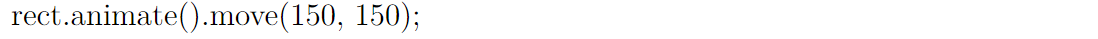
\includegraphics[width=15cm]{img/alg3.PNG}
    \caption{Jednoduchá zmena polohy elementa}
    \label{alg3}
\end{figure}

Metóda animate() bude mať tri argumenty. Prvým je duration, druhým  delay a tretím  when. Prípadne, môžeme odovzdať objekt ako prvý argument, ktorý akceptuje  aj viac parametrov  (Obrázok \ref{alg4}).

\begin{figure}[!htbp]
    \centering
    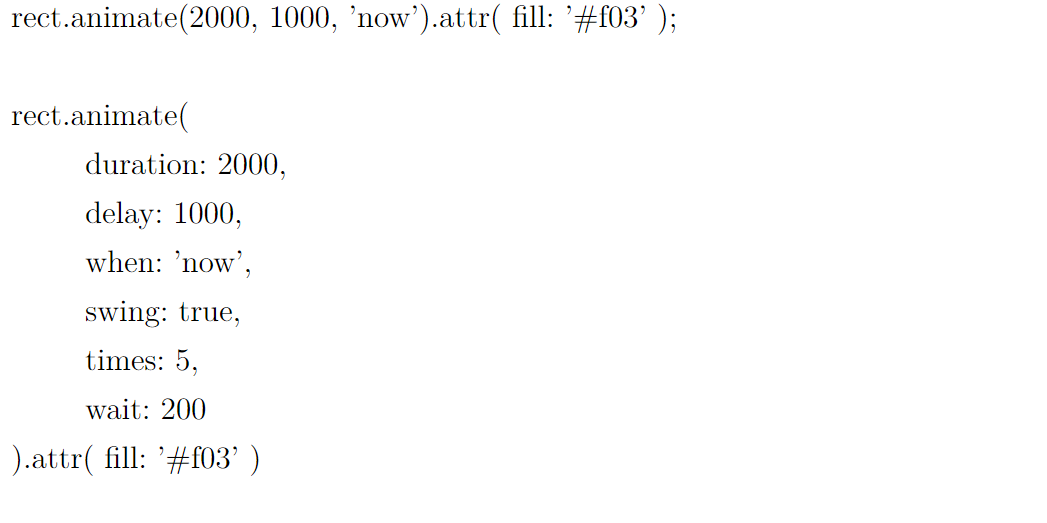
\includegraphics[width=15cm]{img/alg4.PNG}
    \caption{Animovanie zmeny farby obdĺžnika}
    \label{alg4}
\end{figure}

Parameter duration nastaví dĺžku animácie na zadané číslo v milisekundoch. Parameter delay nastaví oneskorenie animácie. Delay je užitočný pri spúšťaní viacero animácií naraz. Parameter when špecifikuje kedy sa má animácia spustiť. Parameter when je predstavený vo forme reťazca, ktorý akceptuje kľúčové slová „now“, „absolute“, „relative“ alebo „last“. Najčastejšie sa používa kľúčové slovo „now“, ktoré špecifikuje, že okamžite chceme spustiť animáciu, lebo oneskorenia sa ľahko nastavujú pomocou parametra delay. V  predvolenom    nastavení, duration je nastavené na 400, delay je nastavené na 0 a when je nastavené na ’now’. Iné parametre nie je potrebné využiť na tvorbu našich animácií.

\newpage

Metóda animate() nevráti cieľový prvok, ale inštanciu SVG.Runner, ktorá má rovnaké metódy ako ktorýkoľvek prvok, ale má aj vlastné metódy na ovládanie animácie. Preto je vhodne si zachovať tieto elementy vo vhodne pomenovaných premenných. JavaScript nám umožňuje ľahké parsovanie dát (pomocou typu var a let), tak môžeme veľmi ľahko definovať polia, do ktorých vložíme naše animácie (Obrázok \ref{alg5}).

\begin{figure}[!htbp]
    \centering
    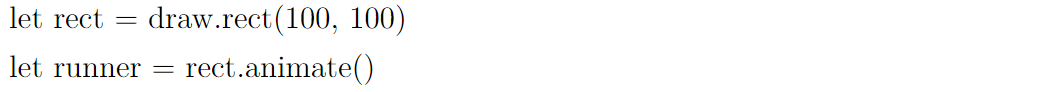
\includegraphics[width=15cm]{img/alg5.PNG}
    \caption{Metóda animate0 vracia inštanciu SVG.Runner}
    \label{alg5}
\end{figure}

Existuje množstvo možností na tvorbu grafov. Najlogickejší spôsob tvorby grafu je využívanie JS knižníc. Existuje veľký počet užitočných knižníc, ale my sme si zvolili plotly.js. Plotly.js je deklaratívna knižnica grafov na vysokej úrovni. Plotly.js pracuje s viac ako 40 typmi máp, vrátane 3D máp, štatistických grafov a \acrshort{SVG}máp [30]. Funguje jednoduchým spôsobom. Potrebné je iba zadefinovať X a Y hodnoty. V našom prípade, budeme mať tri množiny Y hodnôt a desať zadefinovaných bodov. Hneď pri zadefinovaní hodnôt môžeme našim bodom a čiaram prideliť vlastnosti a zapísať ich do premenných. Tento kód môžeme vidieť na obrázku Obrázok \ref{alg6}. 

\begin{figure}[!htbp]
    \centering
    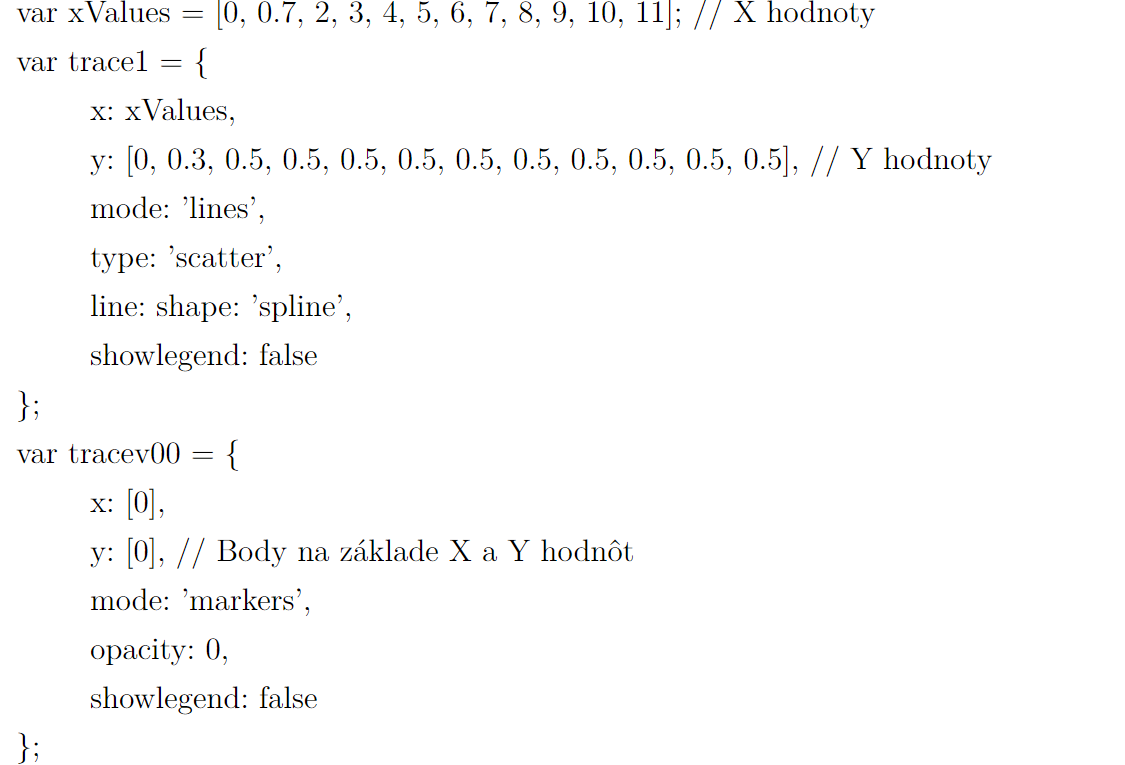
\includegraphics[width=15cm]{img/alg6.PNG}
    \caption{Tvorba čiar a bodov pre graf}
    \label{alg6}
\end{figure}

\newpage \noindent Na základe dát, ktoré sme vytvorili, vytvárame graf pomocou metódy newPlot(), (Obrázok \ref{alg7}). Výsledný graf je možné vidieť na obrázku Obrázok \ref{graf}.

\begin{figure}[!htbp]
    \centering
    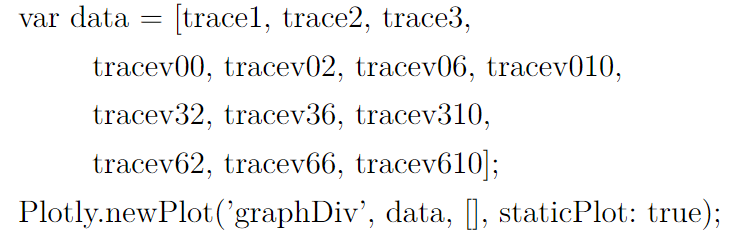
\includegraphics[width=10cm]{img/alg7.PNG}
    \caption{Tvorba dát pre graf}
    \label{alg7}
\end{figure}

\begin{figure}[!htbp]
    \centering
    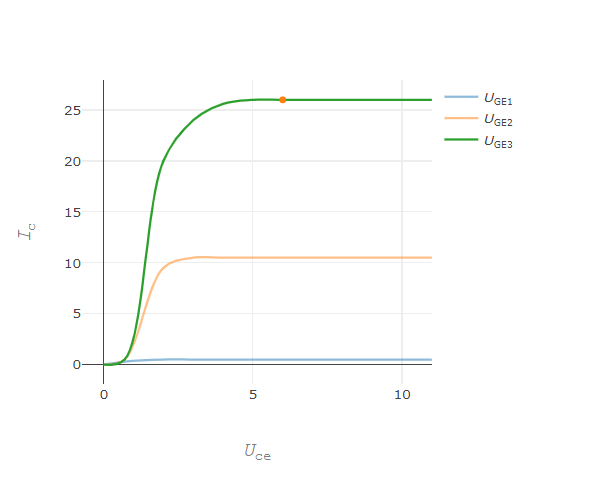
\includegraphics[width=12cm]{img/graf.PNG}
    \caption{Výsledný graf}
    \label{graf}
\end{figure}

Umiestnenie našich animácií do premenných nám umožnilo využívať metódy SVG.Runnera. SVG.Runner má veľa vlastných metód, takže ukážeme iba metódy, ktoré sú vhodné pre  naše animácie. Metóda timeline() vracia alebo nastavuje časovú os našej animácie. To v podstate znamená, že môžeme manipulovať časovou osou našej animácie pomocou užitočných metód akými sú .stop(), .pause() a play(). Metóda animate() nám znovu umožní pridať nejakú inú animáciu k objektu. Metóda loop() nám zacyklí animáciu. Metóda speed() zmení súčasne nastavenú rýchlosť animácie. Metóda during() nám umožňuje pripojenie novej funkcie k našej animácii. Vďaka tomu sa dajú vytvoriť trochu zložitejšie animácie, lebo vieme ovládať pohyb animácií pomocou vlastne vytvorených ciest. V algoritme Algoritmus \ref{alg8} je možné vidieť príklad ako využiť túto zložitú metódu.

\begin{algorithm}
\begin{algorithmic}
\STATE     // Animation
\STATE    for(let j = 0; j < electronCount; j++)\{
\STATE \tab     animanip[k][j] = electronArray[j].animate(\{
\STATE \tab \tab       duration: (k < 4) ? 2400 : 2750,                        // First 4 electrons move slightly faster  
\STATE \tab \tab      delay: (j * 600) + ((k \% 2) * 300) + startUpDelay,      // Starts slightly later
\STATE  \tab \tab      when: 'now',
\STATE \tab     \}).during(function(pos)\{
\STATE  \tab \tab      let eased\_pos = SVG.easing['-'](pos);                   // Smooth animation
\STATE  \tab \tab      let m = path[k].matrixify();                            // Follow a path
\STATE \tab \tab       let p = new SVG.Point(path[k].pointAt(eased\_pos*pathLength[k])).transform(m);
\STATE  \tab \tab      electronArray[j].move(p.x - 10, p.y - 10);              // Center 
\STATE  \tab    \}).loop();
\STATE    \}
\caption{Metóda during(), nám umožňuje priradiť rôzne vlastností k našej animácií}
\label{alg8} 
\end{algorithmic}
\end{algorithm}

V našej vlastnej funkcii sme pridali vlastnosť hladkej animácie pomocou \acrshort{SVG} metóde .easing(). Easing podľa [’-’] znamená, že naša hladkosť bude lineárna. Takisto, sme zadefinovali cestu pohybu našej animácie v tvare polyline (Obrázok \ref{alg3}). Potom sme tie dve vlastností spojili dovedna a pridali k našej animácii. Umožnili sme animovanie rôznych prvkov tak, že sme umiestnili do poľa (Obrázok \ref{alg6}). Pomocou delay: sa nám podarilo animovať každý prvok nášho poľa 600 milisekúnd jeden za druhým. Ak náš delay násobíme s počtom prvkov v poli a dostaneme presné trvanie našej animácie v milisekundách, tak vytvoríme ilúziu, že sa naše prvky neustále pohybujú dokola.

Ďalej je potrebné iba využiť tento poznatok. Keď chceme vymeniť napätie na hradle alebo kolektore, tak budeme volať funkciu, ktorá na základe kombinácií napätí na hradle a kolektore, zavolá zodpovedajúcu funkciu pre ovplyvňovanie animácií. Metódy .play() a.pause() sú výborné pre naštartovanie a zastavovanie animácie, v prípade keď nemáme napätie na hradle alebo kolektore. Metóda .speed() je výborná na zmenu rýchlosti animácie v prípade zmeny napätia na kolektore. Iné ovplyvňovania riešime tak, že znovu zavoláme metódu .animate() pre zodpovedajúce pole.

\subsection{Overenie riešenia}
\noindent Webová stránka a animácia sú v tejto chvíli úplne dokončené (Obrázok \ref{zanimation}). Aby sme si  boli istí, že náš kód má platnú syntax, používame online validátory kódu. Na overenie HTML a CSS sme použili službu CSS W3C. Všetky chyby a upozornenia sme vyriešili. Visual Studio Code má validátor kódu pre syntax JavaScriptu. Zapli sme najkritickejšie upozornenia na overenie kvality kódu a kód sme prefaktorovali, kým všetky upozornenia nezmizli. Výpočet  novej polohy častíc, aktualizácia polohy dráh a ďalšie úkony sa musia uskutočniť medzi zobrazením dvoch snímok; v opačnom prípade môžeme mať pokles snímok. Aby sme skrátili výpočtový čas, znížili sme počet častíc, do takej miery ako sa to dalo, a tiež sme sa snažili vyhnúť používaniu vnorených slučiek v kóde. Animácia s predpätím pozostáva z vyše 200 tvarov SVG; každý z nich je zároveň uzlom Document Object Model. V každom rámci je potrebné aktualizovať približne 200 vlastností týchto uzlov. Je to ďalší problém, ktorý môže spomaliť animáciu; FPS animácie môže klesnúť na starých mobiloch, notebookoch v režime šetrenia energie alebo vo všeobecne pomalých zariadeniach.

\begin{figure}[!htbp]
    \centering
    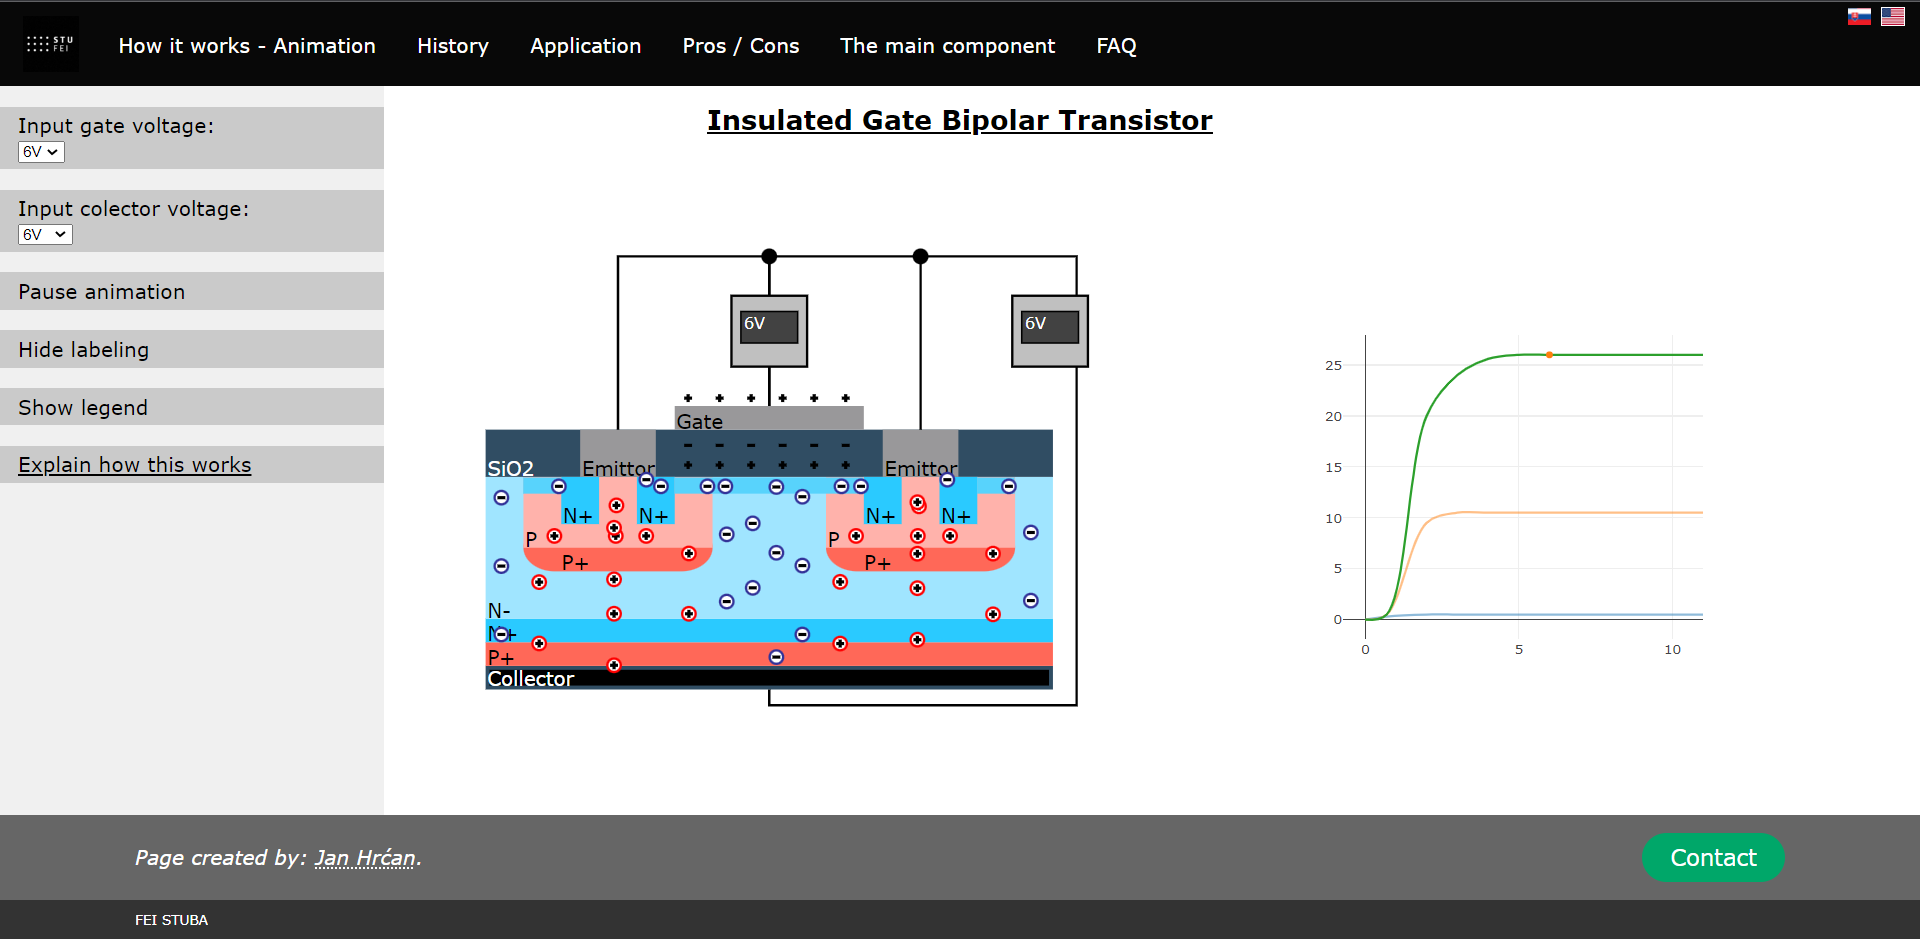
\includegraphics[width=16cm]{img/zanimation.PNG}
    \caption{Výsledná stránka hlavnej animácie}
    \label{zanimation}
\end{figure}

\section{Súhrn}
\noindent V kapitole Súhrn sa budeme venovať realizácií našej stránky tak, že vytvoríme štruktúru a obsah  stránky ako aj každej podstránky. Ukážeme,  akým spôsobom si študent môže vyhľadať žiadané informácie o \acrshort{IGBT} tranzistore a ako môže interagovať s našou stránkou. Aby sa študent dostal k našej stránke, potrebné je buď sa dostať k nej  tak, že  zadá linku umiestenia našej stránky do webového prehliadača, alebo môže stiahnuť celú stránku na vlastný počítač a otvoriť súbor "index.html".

\subsection{Hlavná stránka}
\noindent UML diagram celej aplikácie zobrazuje cestu používateľovi, ako sa dostáť ku jednotlivým položkám (Obrázok \ref{UMLMain}). Na hlavnej stránky su používateľ prečíta krátky opis každej podstránky, aby vedel kde má hľadať žiadané informácie (Obrázok \ref{mainpage}). Intro sme umiestnili do stredu našej hlavnej stránky, aby si používateľ pozrel video, ktoré sme pre neho pripravili. V strede sa nachádza tlačidlo, ktoré načíta a naštartuje naše video. Vo videu sme pripravili krátku prezentáciu s relaxačnou hudbou v pozadí. Obsah  prezentácie tvorí niekoľko snímok, na ktorých e máme popísane niekoľko základných a zaujímavých vlastností \acrshort{IGBT}, so zámerom aby  naše video prilákalo používateľa, aby ďalej pokračoval v sledovaní našej stránky.

\begin{figure}[!htbp]
    \centering
    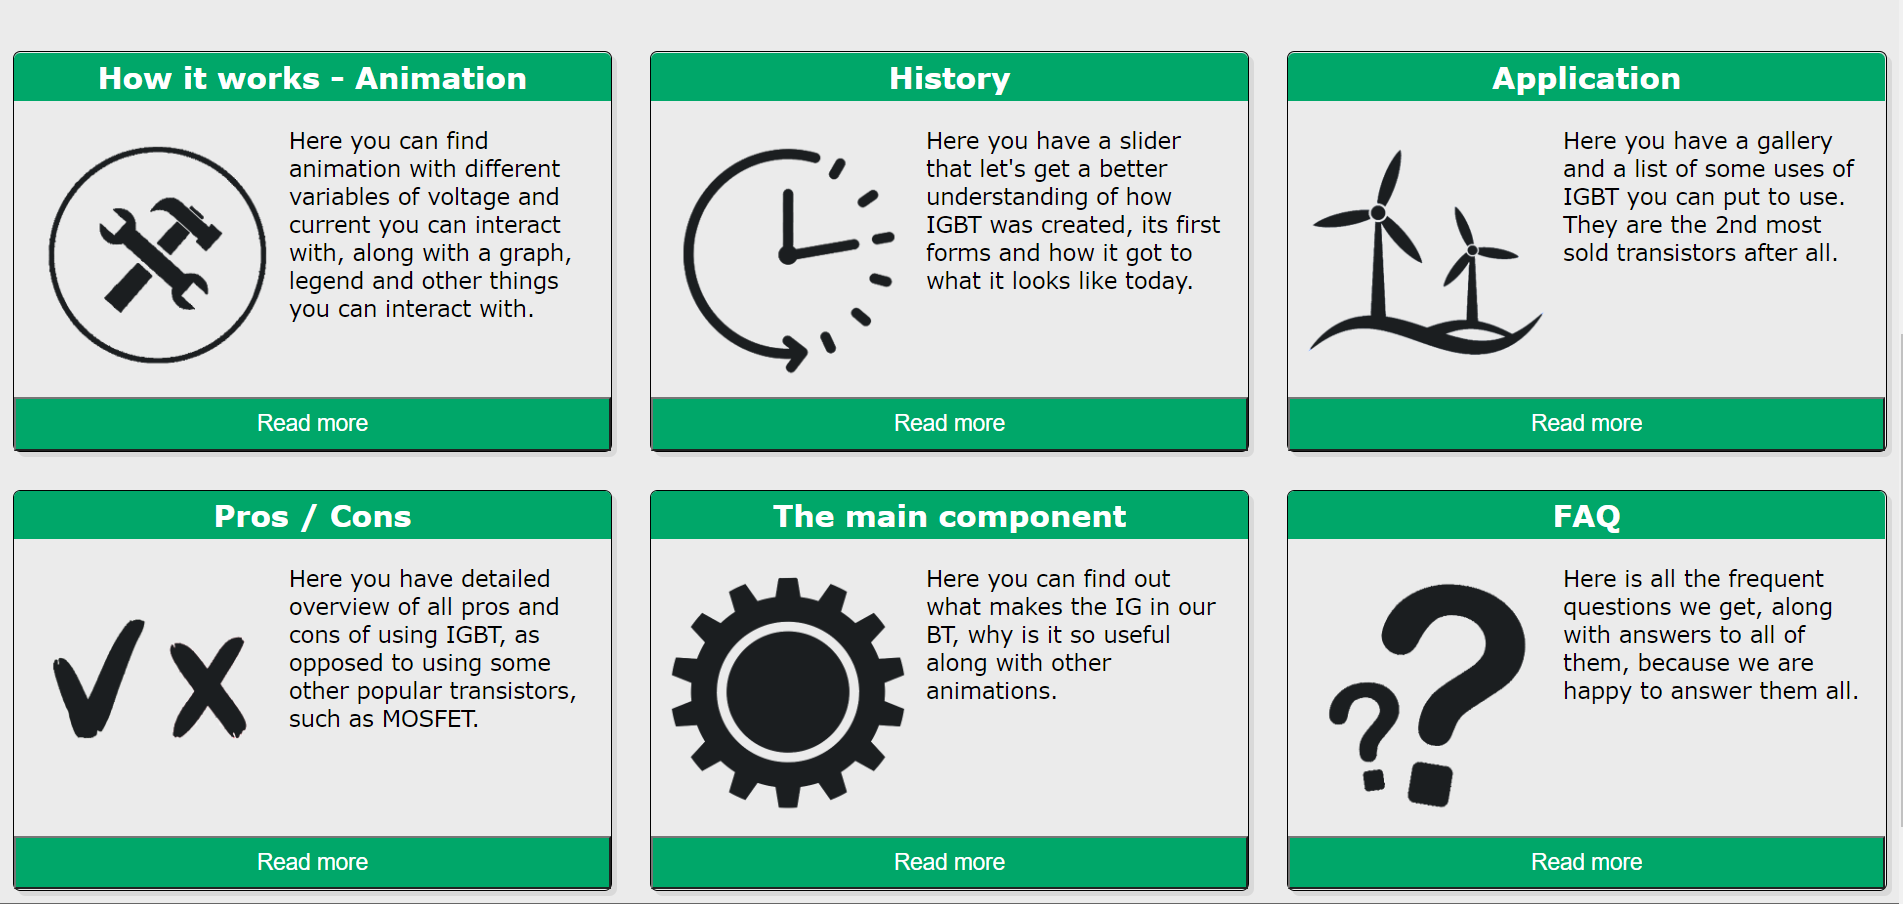
\includegraphics[width=16cm]{img/mainpage.PNG}
    \caption{Hlavná stránka}
    \label{mainpage}
\end{figure}

Po prečítaní obsahu tejto stránky, používateľ by už mal vedieť, čo každá podstránka obsahuje, ako aj vuyžívať aj navigačné menu (Obrázok \ref{navbar}) na prepojenie sa medzi podstránkami. Po kliknutí na logo v navigačnom menu, sa používateľ môže vrátiť späť na domovskú stránku. V pravom hornom rohu sa nachádzajú vlajky Slovenska a USA. Po kliknutí na vybranú vlajku, obsah stránky sa preloží na slovenský alebo anglický jazyk. Taktiež je uvedené zachovanie predvoleného jazyka vo webovom skladisku. Štruktúru tejto stránky sme realizovali v podobe mriežky, ktorá je prednastavená zobraziť hlavné menu v maticovej podobe $2\times 3$ (2 rady, 3 stĺpce). Na menších obrazovkách tá matica bude $3\times 1$ a na najmenších obrazovkách to bude $6\times 1$.

\begin{figure}[!htbp]
    \centering
    
\includegraphics[width=16cm]{img/navbar.PNG}
    \caption{Navigačné menu stránky}
    \label{navbar}
\end{figure}

\subsection{Princíp činnosti}
\noindent Na podstránke Princíp činnosti sme si umiestnili našu hlavnú animáciu (Obrázok \ref{pc}). Na ľavej strane sa nachádza bočné menu s rôznymi možnosťami na nastavovanie animácie. Najprv, používateľ si môže zvoliť rozličné hodnoty napätia medzi hradlom a kolektorom. Predvolené hodnoty napätia medzi hradlom a kolektorom sú  6 V. Akonáhle používateľ zmení hodnoty, tak sa niečo  zmení v animácii (napríklad: animácia sa spomalí ak používateľ zadá 3 V medzi emitorom a kolektorom a 3 V alebo 6 V medzi hradlom a emitorom). Takisto je možné pozastaviť animácie stlačením na tlačidlo "Pozastav animáciu". Opätovné stlačenie tohto tlačidla nám umožní pokračovať v ukážke animácie. Používateľ môže takisto skryť a znázorniť označenia na obrázku \acrshort{IGBT} tranzistora ako aj skryť alebo znázorniť legendu. Na konci sa nachádza linka na podstránku teórie IGBT, kde je pomocou textu a obrázkov vysvetlené ako \acrshort{IGBT} tranzistor funguje. Tu sme takisto využili mriežkovú štruktúru pre vizualizáciu obsahu stránky. Ak používateľ má malú obrazovku, tak graf a animácia  budú jeden nad druhým, namiesto vedľa seba.


\begin{figure}[!htbp]
    \centering
    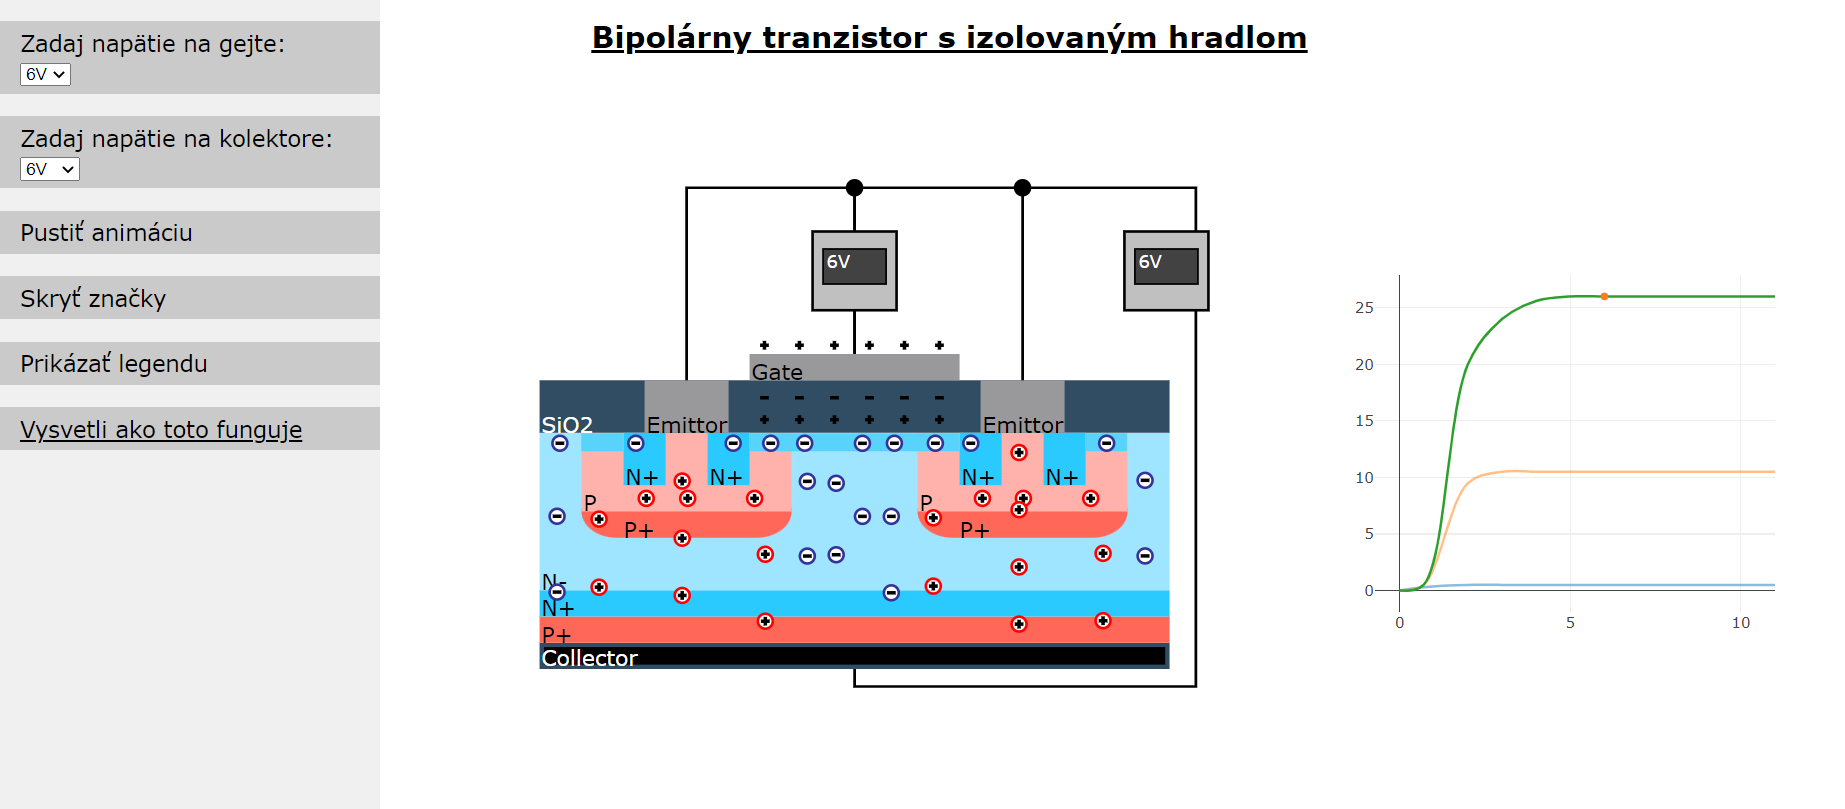
\includegraphics[width=16cm]{img/pc.PNG}
    \caption{Princíp činnosti IGBT}
    \label{pc}
\end{figure}

\subsection{História}
\noindent V historickom okienku sa nachádza krátka prezentácia vývoja \acrshort{IGBT} tranzistora (Obrázok \ref{history}). Používateľ je schopný sa prepnúť medzi snímkami tak, že posúva guľôčku na slideri vľavo alebo vpravo, alebo môže použiť šípky na klávesnici. Takúto  interaktivitu  sme zrealizovali pomocou CSS. Všetky obrázky sú vedľa seba, ale okienko, v ktorom sú umiestnené obrázky, má veľkosť iba jedného obrázku. Na základe hodnoty slidera, pomocou JS posúvame okraj prvého obrázku tak, aby sa na obrazovku dostal žiadaný obrázok.

\newpage

\begin{figure}[!htbp]
    \centering
    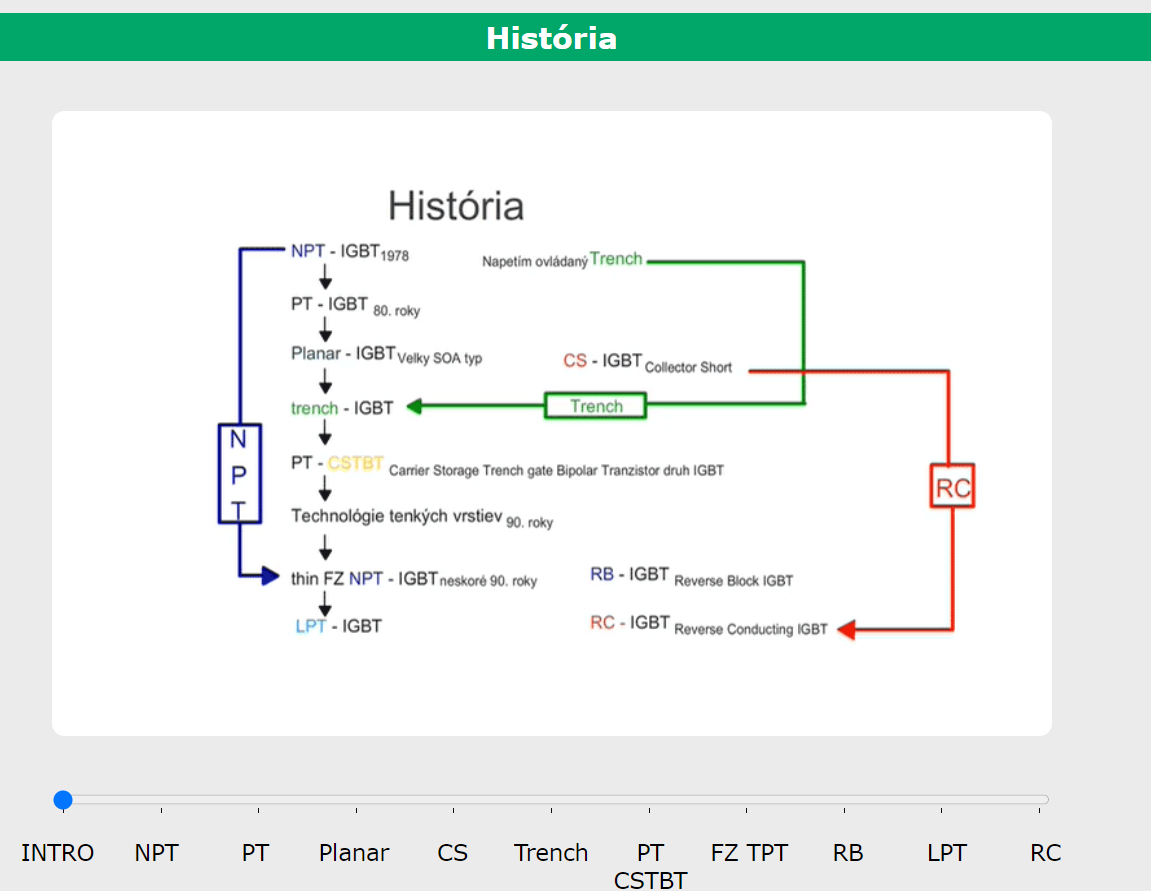
\includegraphics[width=16cm]{img/history.PNG}
    \caption{Historické okienko IGBT}
    \label{history}
\end{figure}

V historickom okienku sa prvýkrát stretávame s ikonkou zdrojového súboru (Obrázok \ref{src}). Môžeme ho nájsť na rôznych stránkach. Po kliknutí na túto ikonku si otvoríme všetky citácie zdrojových súborov, použitých na vyplnenie obsahu stránky, na ktorej sa používateľ momentálne nachádza.

\begin{figure}[!htbp]
    \centering
    
\includegraphics[width=5cm]{img/src.PNG}
    \caption{Ikonka zdrojového súboru}
    \label{src}
\end{figure}

\subsection{Aplikácie}
\noindent Na stránke aplikácie používateľ uvidí krátku prezentáciu niektorých použití \acrshort{IGBT} tranzistora (Obrázok \ref{app}). Stránka obsahuje stručnú informáciu o tom, ako sa dá použiť \acrshort{IGBT} tranzistor, a potom používateľ môže posúvať slider aby videl iné snímky prezentácie. Ako používateľ mení snímku na obrazovke, tak sa mení druhá časť popisu, ktorá popisuje akú úlohu \acrshort{IGBT} má v danom príklade. Túto krátku prezentáciu sme vytvorili pomocou príkladu JS a CSS kódu, ktorý je zobrazený na stránke w3schools.com. Takisto sa znovu môžeme stretnúť s mriežkovou štruktúrou. Ak používateľ má malú obrazovku, tak prezentácia a popis budú jedno nad druhým, namiesto vedľa seba.

\begin{figure}[!htbp]
    \centering
    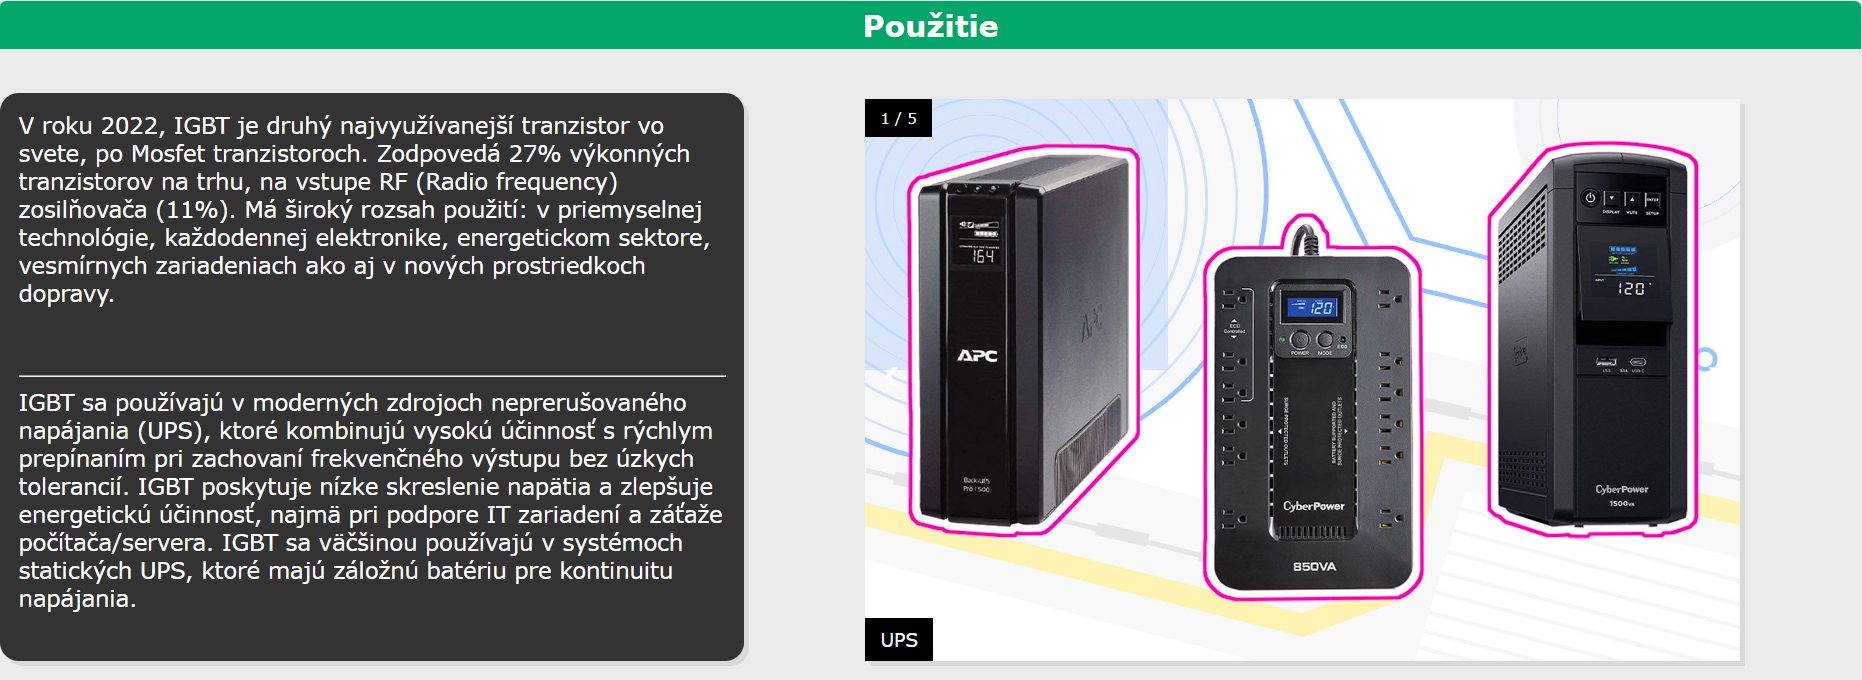
\includegraphics[width=16cm]{img/app.PNG}
    \caption{Ukážka z animácie použitia IGBT}
    \label{app}
\end{figure}

\subsection{Výhody/Nevýhody}
\noindent Na stránke Výhody/Nevýhody sa nachádzajú dva jednoduché a krátke zoznamy, ktoré popisujú výhody, respektíve nevýhody \acrshort{IGBT} tranzistora. Tu je taktiež jednoduché mriežkové zobrazenie, aby sme mohli vidieť výhody a nevýhody jeden vedľa druhého.

\subsection{Teória IGBT}
\noindent Stránka teórie IGBT má dva hlavné ciele. Ako sám názov hovorí, cieľom tejto stránky je vysvetliť a popísať ako funguje IGBT. Takisto, cieľom tejto stránky je slovom a obrázkom vysvetliť ako \acrshort{IGBT} tranzistor funguje. Na tejto stránke sa nachádza krátka prezentácia toho, čo sa deje v \acrshort{IGBT} tranzistore, aby \acrshort{IGBT} sa zopol. Používateľ znovu môže použiť slider na prepájanie sa medzi jednotlivými snímkami, pričom každá snímka má svoj vlastný popis (Obrázok \ref{main}). V dolnom ľavom rohu sa nachádza tlačidlo, ktoré nás odvedie späť ku hlavnej animácii. Ak používateľ má malú obrazovku, tak prezentácia a popis budú jedno nad druhým, namiesto vedľa seba.

\begin{figure}[!htbp]
    \centering
    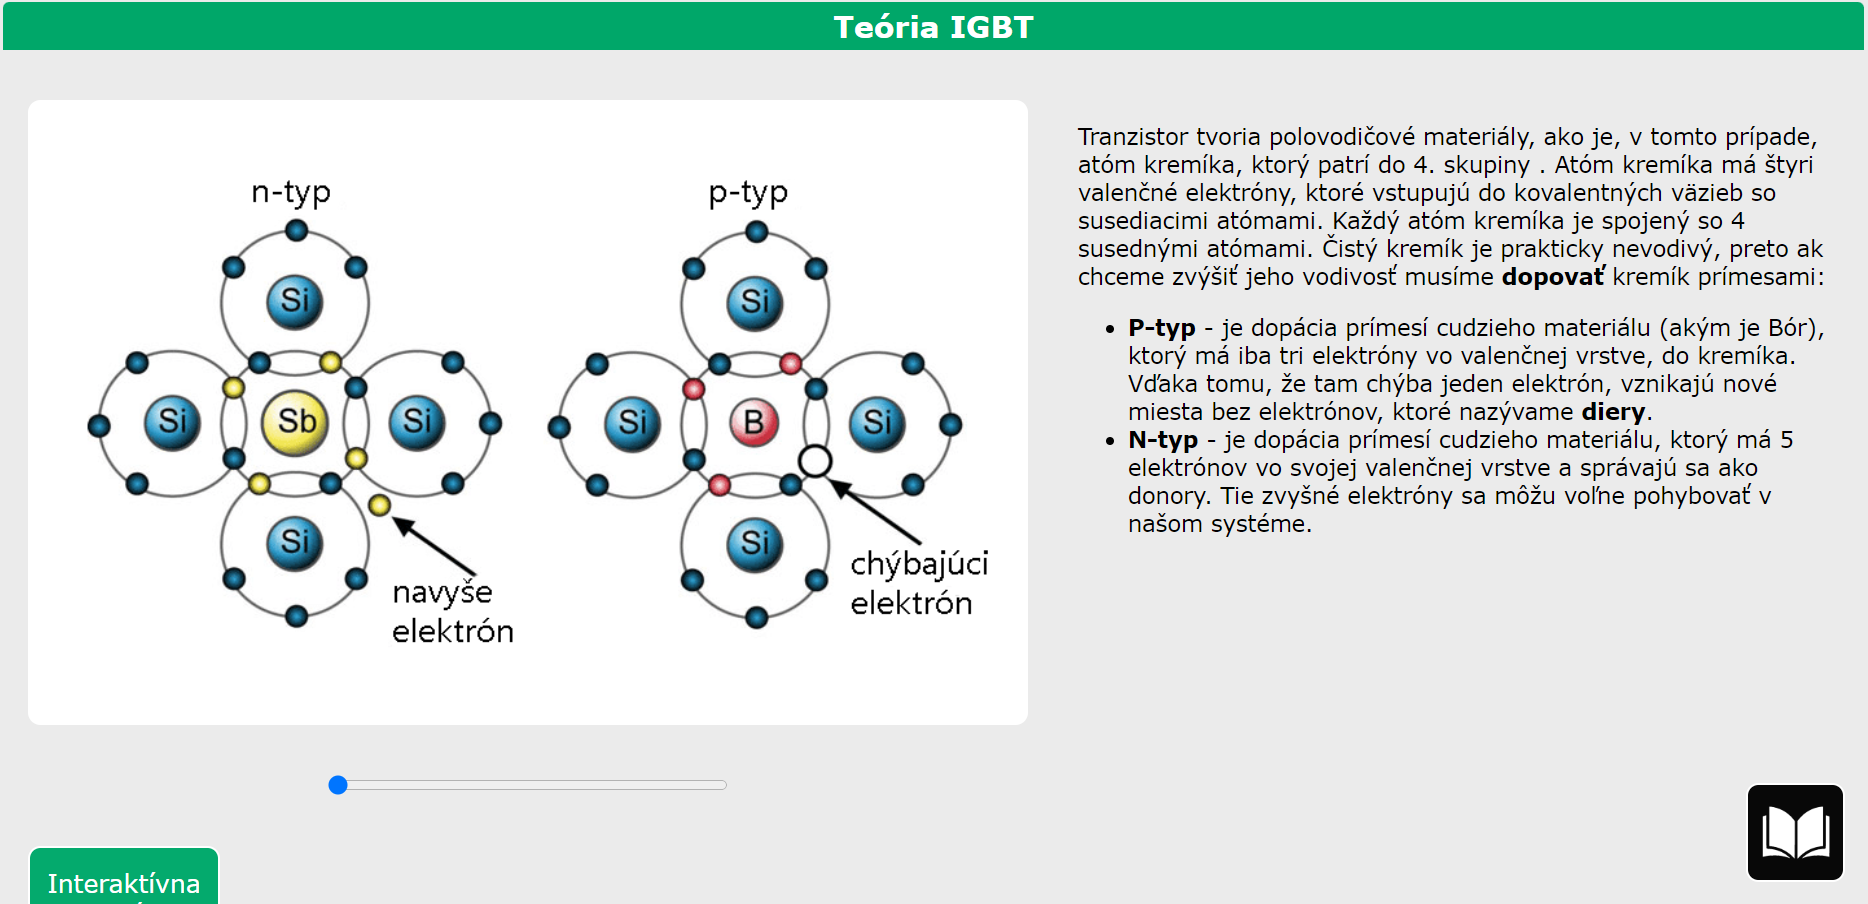
\includegraphics[width=16cm]{img/main.PNG}
    \caption{Ukážka stránky teorií IGBT}
    \label{main}
\end{figure}

\subsection{FAQ}
\noindent Frequently Asked Questions je stránka, ktorá je plánovaná ako predvolené miesto pre používateľa aby kládol otázky. Na tejto stránke sa už nachádza niekoľko otázok  a odpovedí, ktoré by používateľa prípadne zaujímali. Ak sa používateľ rozhodne položiť otázku, tak otázka bude odoslaná na univerzitný mail a budeme sa snažiť na ňu odpovedať. Akonáhle prečítame prijatú otázku,  aktualizujeme stránku s odpoveďou na ňu. Zrealizovali sme to za pomoci jednoduchého formulára, ktorý komunikuje so zadaným emailom.

\section{Technická dokumentácia}
\noindent V kapitole Technická dokumentácia objasníme ako tento projekt funguje na počítači, ako súbory komunikujú medzi sebou a akú úlohu má každý súbor. \newline

Dôležité je si uvedomiť, že táto stránka sa zobrazuje ako webová aplikácia, takže na jej prehliadanie je potrebné mať webový prehliadač. Pretože táto práca je vytvorená pomocou štandardu HTML5, tak animácia bude fungovať iba na nasledovných prehliadačoch: GoogleChrome (verzia 52 a nahor), Mozilla Firefox (verzia 54 a nahor), Opera (verzia 39 a nahor), Safari (verzia 10.1 a nahor) a Microsoft Edge (verzia 14 a nahor). Na starších, alebo nespoľahlivých prehliadačoch, ako je Internet Explorer, táto aplikácia nebude funkčná.

Desktopová verzia webovej stránky sa spúšťa kliknutím na súbor index.html. V hlavnom súbore sa nachádzajú všetky naše stránky, pokiaľ index.html predstavuje začiatočnú stránku. Index.html je rezervované meno stránky, tak prehliadače prečítajú index.html súbor po návšteve linky stránky. CSS súbory sú umiestnené v CSS priečinku a JS súbory sú umiestnené v JS priečinku.

Aby CSS kód bol transparentnejší, každej stránke sme vytvorili vlastný .css súbor. Hlavný  súbor je style.css, ktorý využívajú všetky stránky. Ak chceme vymeniť vlastnosť jedného elementu v nejakom .css súbore, ktorý má inakšiu vlastnosť v hlavnom súbore, tak sa tá vlastnosť vymení iba pre tú stránku, ktorá využíva ten .css súbor.

Aby Javascriptový kód bol transparentnejší, každá podstránka (celkovo ich je 6) má svoj vlastný .js súbor a ten má rovnaký názov ako html súbor, ktorý uvedený .js súbor má ovplyvňovať (napríklad apps.html využíva app.js). Každá stránka môže využívať nekonečne veľa .js súborov, potrebujeme iba zavolať lokálnu linku na požadovaný súbor (linku v počítači) alebo webovú linku. Hlavný .js súbor \textit{script.js} využívajú všetky stránky, lebo sa tu nachádza kód, ktorý umožňuje zobrazenie obsahu stránok v slovenčine alebo angličtine. 

Tu je potrebné si uvedomiť, že obsah všetkého textu sa nachádza v súbore \textit{script.js} alebo \textit{script-work-language.js}, tak ak by niekto chcel upraviť text, musel by ho meniť v Javascriptovom súbore. V oboch prípadoch, algoritmus funguje rovnako; celý obsah stránok sa nachádza v .JSON objekte, ktorý má dva polia, len a lsk (anglícky a slovenský text). Tie majú rovnaké premenné, ktoré sú pomenované podľa id, ktoré ho majú ovplyvňovať. Tak stačí sa pozrieť na id nejakého html elementu, ktorému chceme upraviť text, a jeho zdrojový text nájdeme v .JSON objekte pod rovnakým menom. 

Pre niektoré zložitejšie podstránky sme vytvorili viac .js súborov, lebo JavaScript súbory môžu navzájom komunikovať.  Stránka work má štyri Javascript súbory. Vo \textit{script-word-draw.js} kreslíme \acrshort{SVG}objekty, vo \textit{script-work-language.js} nastavujeme jazyk po voľbe predvoleného jazyka, vo \textit{script-work-graph.js} kreslíme graf a vo \textit{script-work.js} vytvárame animácie a využívame funkcie všetkých spomenutých .js súborov. Takisto, v tomto priečinku sa nachádzajú súbory knižnice SVG.js, ktoré umožňujú využívanie služieb na kreslenie a animovanie. Súbor \textit{script.main-animation.js} v sebe obsahuje kód pre animovanie dvoch animácií v \textit{main.html} súbore. 

Taktiež, máme súbor \textit{source.js}, ktorý obsahuje kód na zobrazenie a skrývanie zdrojov pre  stránky, ktoré to využívajú.

\subsection{Animácia}
\noindent Súbor \textit{svg.js}, ktorý sme stiahli zo stránke svgjs.dev/docs/3.0/installation/ je nutný pri vytváraní animácií, lebo už obsahuje kód a funkcie, ktoré nám umožnili ľahšie naprogramovanie naších animácií. Ako sme si už vysvetlili v druhej kapitole, tento súbor nám poskytuje funkcie na kreslenie (ako je draw()) a funkcie na animovanie (ako je animate()). 
Každý krok v kóde a každá premenná je dobre okomentovaná. Dôležité je si uvedomiť, že na začiatku sme si zadefinovali polia, do ktorých uložíme naše SVG objekty. Takisto máme zadefinované pole \textit{animanip[]}, do ktorého uložíme každú animáciu, ktorú planujeme ovplyvňovať. Zostávajúce veci sme si už vysvetlili v práci a v komentároch v kóde.